%pdflatex --shell-escape scap_benchmark_dl_training_results
%biber scap_benchmark_dl_training_results

\PassOptionsToPackage{hyphens}{url}
\documentclass[compress,aspectratio=169]{beamer}

\usepackage[official]{eurosym}
\usepackage{multirow}
\setlength{\marginparwidth}{2cm}
\usepackage{todonotes}
\presetkeys{todonotes}{inline}{}
\usepackage[style=verbose,backend=biber,style=authoryear, citestyle=authoryear ]{biblatex}
\setbeamertemplate{bibliography item}{\insertbiblabel} % Ensure that cite labels appear in references section
\addbibresource{ref.bib}
\usepackage{../assets/beamerthemeGoettingen} % make sure the theme file is on this path
\graphicspath{{../}{../assets/}}
\usepackage{caption}
\usepackage{booktabs}

\usepackage{listings}
\lstset{
    autogobble,
    columns=fullflexible,
    showspaces=false,
    showtabs=false,
    breaklines=true,
    showstringspaces=false,
    breakatwhitespace=true,
    escapeinside={(*@}{@*)},
    commentstyle=\color{greencomments},
    keywordstyle=\color{bluekeywords},
    stringstyle=\color{redstrings},
    numberstyle=\color{graynumbers},
    basicstyle=\ttfamily\footnotesize,
    frame=l,
    framesep=12pt,
    xleftmargin=12pt,
    tabsize=4,
    captionpos=b
}

\usepackage{fancyvrb}
\usepackage[normalem]{ulem}

\hypersetup{
    colorlinks,
    citecolor=black,
}

\newcommand{\source}[1]{\par\begin{textblock*}{6cm}(1cm,8cm)
    \begin{beamercolorbox}[wd=\paperwidth,ht=0.5cm,right]{framesource}
        \usebeamerfont{framesource}\usebeamercolor[fg]{framesource} \centering\tiny {#1}
    \end{beamercolorbox}
\end{textblock*}}


% listing / code
\usepackage{minted}
\usemintedstyle{tango}
% Box listing / code
\usepackage{tcolorbox}

% Box listing / code style 
% These options will be applied to all `tcolorboxes`
\tcbset{%
    noparskip,
    colback=gray!5, %background color of the box
    colframe=gray!20, %color of frame and title background
    coltext=black, %color of body text
    coltitle=black, %color of title text 
    fonttitle=\tiny,
    alerted/.style={coltitle=red, 
                     colframe=gray!40},
    example/.style={coltitle=black, 
                     colframe=green!20,             
                     colback=green!5},
    }

\lstset{literate=%
    {Ö}{{\"O}}1
    {Ä}{{\"A}}1
    {Ü}{{\"U}}1
    {ß}{{\ss}}1
    {ü}{{\"u}}1
    {ä}{{\"a}}1
    {ö}{{\"o}}1
    {~}{{\textasciitilde}}1
}

\usepackage{csquotes} % For \enqoute{}
\usepackage{hyperref}

\usepackage{xcolor}
\definecolor{c1}{HTML}{ed5151}
\definecolor{c2}{HTML}{149ece}
\definecolor{c3}{HTML}{a7c636}
\definecolor{c4}{HTML}{9e559c}
\definecolor{c5}{HTML}{fc921f}
\definecolor{c6}{HTML}{ffde3e}

\usepackage[multiple]{footmisc} %https://tex.stackexchange.com/questions/28465/multiple-footnotes-at-one-point

\newcommand{\backupbegin}{
   \newcounter{framenumberappendix}
   \setcounter{framenumberappendix}{\value{framenumber}}
}
\newcommand{\backupend}{
   \addtocounter{framenumberappendix}{-\value{framenumber}}
   \addtocounter{framenumber}{\value{framenumberappendix}} 
}

% --- document configuration ---
\newcommand{\mytitle}{Profiling tree species classification\\with synthetic data and deep learning}     
% Leave empty for no subtitle
\newcommand{\mysubtitle}{State of the art and plan for Scalable Computing Systems and Applications in AI, Big Data and HPC}   
\newcommand{\myauthor}{Hauke Kirchner}
\newcommand{\myauthorurl}{\href{http://www.overleaf.com}{Something 
Linky}}
\newcommand{\myvenue}{Göttingen}
% For example, use \today
\newcommand{\mydate}{2.2.2023}
% For example, Institute for Computer Science / GWDG
\newcommand{\myinstitute}{GWDG - AG Computing}
% Leave empty for no footer image
\newcommand{\myfooterimage}{}           
\newcommand{\mygrouplogo}{}
% Images must be enabled manually under title page \titleLogo
% Adjust position and width manually for fewer images
\newcommand{\mytitleimageone}{}         
\newcommand{\mytitleimagetwo}{}        
\newcommand{\mytitleimagethree}{}

% --- title page ---
\title{\Large \mytitle}
\venue{\myvenue}
\date{\mydate}
\subtitle{\mysubtitle}
%\authorURL{\myauthorurl}
\author{{\myauthor}}
\authorFooter{\myauthor \hspace{0.3cm} \includegraphics[height=1em]{\myfooterimage}}
\institute{\myinstitute}
\groupLogo{\includegraphics[width=2cm]{\mygrouplogo}}
\titleLogo{
%\includegraphics[height=2.7cm]{\mytitleimageone}
%\includegraphics[height=2.7cm]{\mytitleimagetwo}
%\includegraphics[height=2.7cm]{\mytitleimagethree}
}

\setbeamertemplate{footline}[text line]{
\begin{beamercolorbox}[sep=0.5em,wd=\paperwidth,leftskip=0.2cm,rightskip=0.1cm]{footlinecolor}
\myauthor \hfill \insertVenue \hfill \insertframenumber\,/\,\ref{pg:lastpage}
\end{beamercolorbox}
}

\begin{document}

\begin{frame}[plain]
	\titlepage
\end{frame}

\begin{frame}[t]{Table of contents}
  \tableofcontents[subsectionstyle=hide/hide]
\end{frame}

% --- slides begin ---

\section{Research Goals}

\iffalse
\begin{frame}{Why is it important to profile\\the training process of neural networks?}

    \begin{columns}
        \begin{column}{0.5\textwidth}
            \begin{block}{\centering Training speed}
                \centering
                \vspace{3em}
                
\includegraphics[width=0.3\textwidth]{assets/speed_FILL0_wght400_GRAD0_opsz48.png}
            \end{block}
        \end{column}
        \begin{column}{0.5\textwidth}
            \begin{block}{\centering Energy efficiency}
                \centering
                \vspace{3em}
                
\includegraphics[width=0.3\textwidth]{assets/electric_bolt_FILL0_wght400_GRAD0_opsz48}
            \end{block}
        \end{column}
    \end{columns}

\end{frame}

\begin{frame}{Training speed 
              \begin{tabular}{@{}c@{}}
                  
\includegraphics[width=0.05\textwidth]{assets/speed_FILL0_wght400_GRAD0_opsz48.png}
              \end{tabular}
              }

    \vspace{-3em}

    \begin{columns}
        \begin{column}{0.6\textwidth}
            \begin{itemize}
                \item training of neural networks is computationally intensive
                \vspace{1em}
                \item[$\hookrightarrow$] optimizations for available hardware
                    \begin{itemize}
                        \item How to make good use of clusters with heterogenous hardware?
                        \item How many GPUs are worth requesting?
                    \end{itemize}
            \end{itemize}
        \end{column}
        \begin{column}{0.4\textwidth}
            \vspace{-1em}
            \begin{figure}
                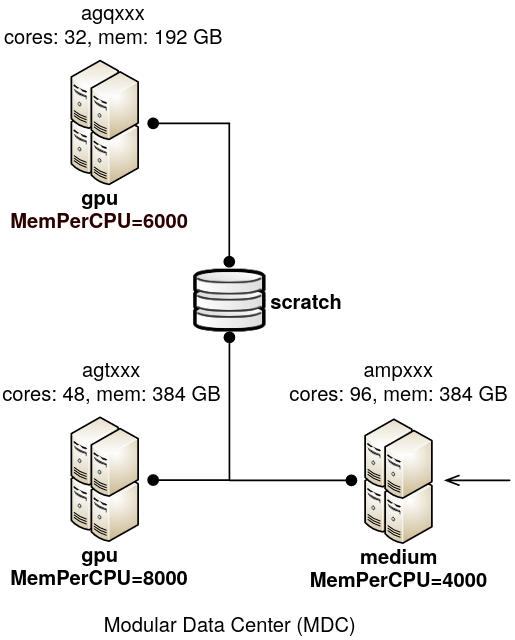
\includegraphics[width=0.9\textwidth]{assets/gwdg_scc.png}
                \caption*{Structure and resources of a part of the Scientific Compute Cluster (SCC).}
            \end{figure}
        \end{column}
    \end{columns}

    \source{Image source: Adapted from \url{https://www.gwdg.de/web/guest/hpc-on-campus/scc}, accessed on: 09.11.2022}
\end{frame}

\begin{frame}{Energy efficiency 
              \begin{tabular}{@{}c@{}}
                  
\includegraphics[width=0.05\textwidth]{assets/electric_bolt_FILL0_wght400_GRAD0_opsz48}
              \end{tabular}
              }



    \begin{columns}
        
        \begin{column}{0.6\textwidth}
            \begin{itemize}
                \item for different applications, the required energy ranges from
                    \begin{itemize}
                        \item low demands (finetuning) to
                        \item high demands (training)
                    \end{itemize}
                \vspace{1em}
                \item[$\Rightarrow$] impact on our climate is growing
            \end{itemize}
        \end{column}

        \begin{column}{0.4\textwidth}
            \vspace{-3.5em}
            \centering
            \begin{figure}
            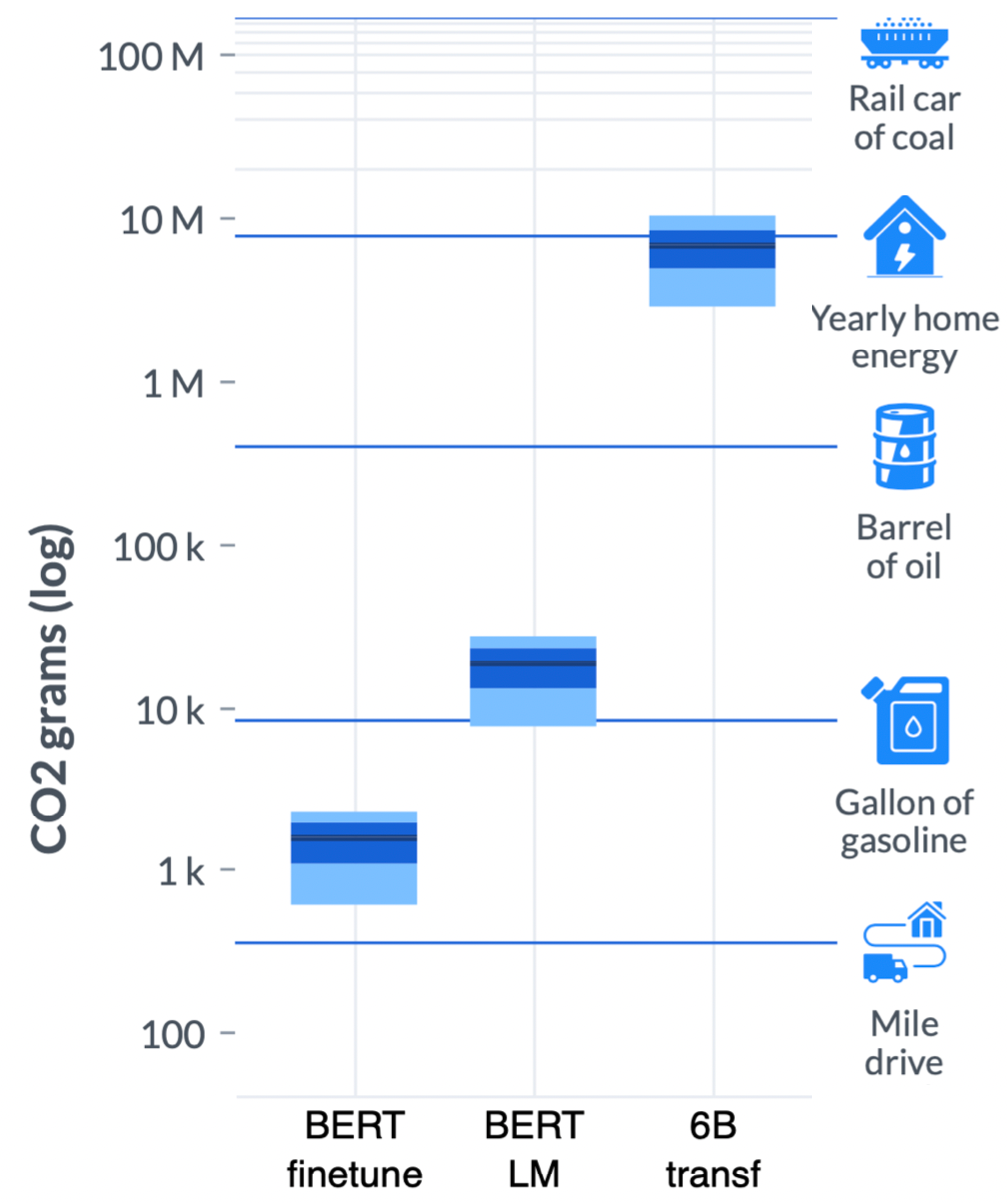
\includegraphics[width=\textwidth]{assets/20220610_dodge_measuring-the-carbon-intensity-of-ai-in-cloud-instances-fig2-bert.png}
            \caption*{$CO_2$ Relative Size Comparison}
            \end{figure}
            \source{Image source: Adapted from \cite{20220610_dodge_measuring-the-carbon-intensity-of-ai-in-cloud-instances}}
            
        \end{column}
    \end{columns}



\end{frame}
\fi
\begin{frame}{Research Goals}

\begin{itemize}
    \item Identify \textbf{profiling tools} that can help to \textbf{optimize an existing PyTorch workflow}.
    \vspace{1em}
    \item As this approach should help scientists, the \textbf{usibility is of high importance}. The simplest tool for doing the job is preferred.
    \vspace{1em}
    \item In contrast to training benchmark suites, such as MLPerf, I do not focus on benchmarking hardware but on optimizing an existing PyTorch workflow (viewpoint of a scientist).
\end{itemize}

\end{frame}

\section{Methods}
%\sectionIntroHidden % Show an outline of the current section with hidden subsections
\sectionIntro % Show an outline of the current section with subsections

\begin{frame}{Tree species classification}
    \begin{columns}
        \begin{column}{0.5\textwidth}

            \begin{block}{Pre-training with synthetic data}
                \begin{enumerate}
                    \item scene generation with Arbaro\footnote{\tiny{\url{https://github.com/wdiestel/arbaro}}}
                    \vspace{1em}
                    \item synthetic lidar data generation with Helios++ (\cite{9906068})
                    \vspace{1em}
                    \item pre-training of\\PointNet (\cite{pointnet})
                    \vspace{1em}
                \end{enumerate}
            \end{block}

        \end{column}
        \begin{column}{0.5\textwidth}
                \centering
                \vspace{-4em}
                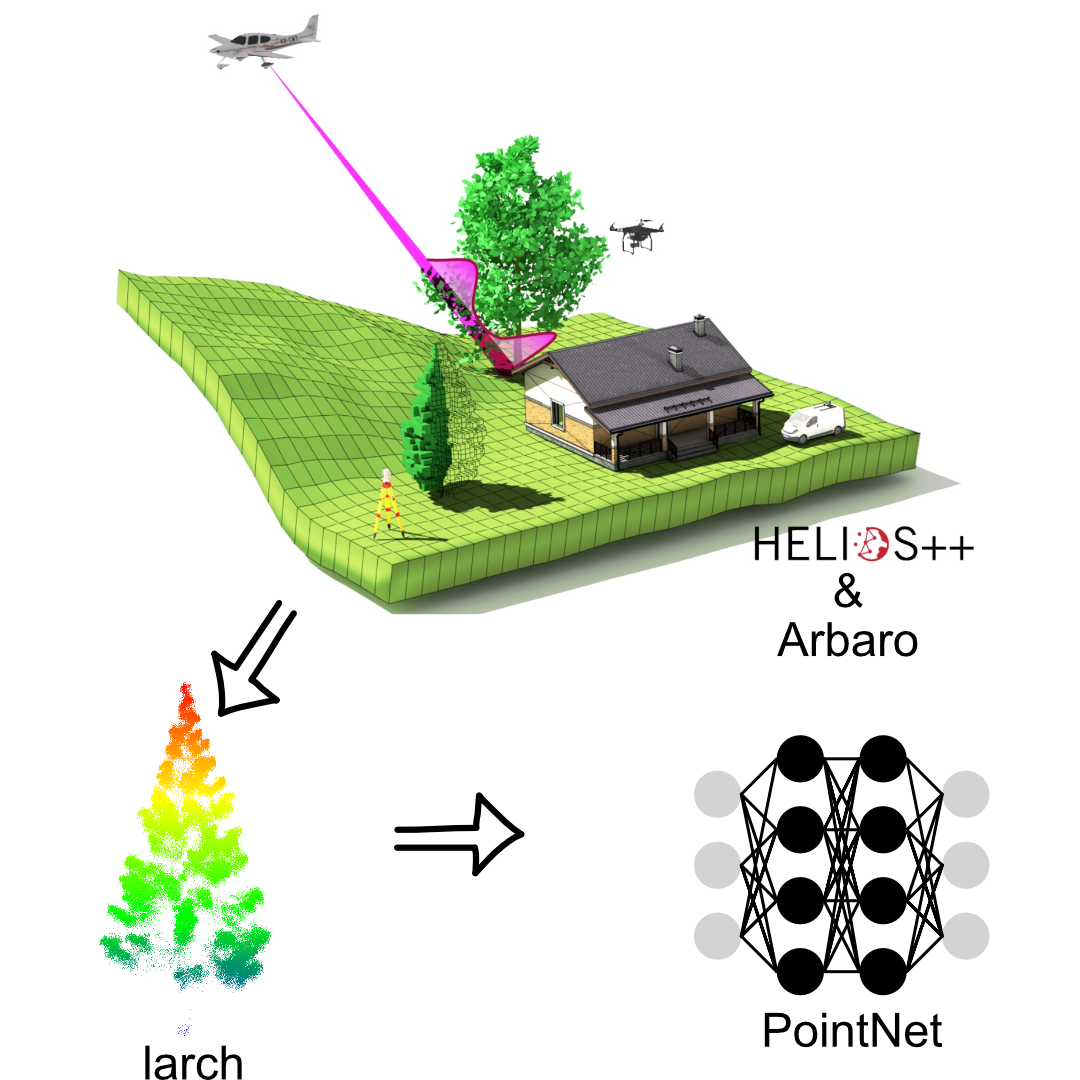
\includegraphics[width=\textwidth]{assets/workflow_synthetic_data}
                \source{Image source: Adapted from \cite{9906068}}
        \end{column}
    \end{columns}
\end{frame}

\begin{frame}{Metrics}

% Please add the following required packages to your document preamble:
% \usepackage{booktabs}
% \usepackage{multirow}
\begin{table}[]
\begin{tabular}{@{}ll@{}}
\toprule
metric                                                                                 & purpose                        \\ \midrule
Execution time                                                                         & \multirow{2}{*}{traditionally} \\
FLOPS                                                                                  &                                \\ \midrule
Throughput: $\frac{images}{sec}$                                                       & with the advent of GPUs        \\ \bottomrule
\end{tabular}
\end{table}


\source{Image source: Adapted from \url{https://snehilverma41.github.io/Metrics_ML_FastPath19.pdf}}

\end{frame}

\begin{frame}[t]{Tools}
    \begin{center}
        
\includegraphics[width=1\textwidth]{../../data/tools}
    \end{center}
    \begin{columns}[t]
    \begin{column}{0.5\textwidth}
                \begin{itemize}
                    \item PyTorch - Profiler~\footnote{\tiny{\url{https://pytorch.org/tutorials/intermediate/tensorboard_profiler_tutorial.html}}}
                    \item collection of performance metrics
                    \item indentification of\\expensive operators
                    \item tracking of the kernel activity
                \end{itemize}
    \end{column}
    \begin{column}{0.5\textwidth}
                \begin{itemize}
                    \item FlopsProfiler~\footnote{\tiny{\url{https://www.deepspeed.ai/tutorials/flops-profiler/}}}
                    \item model speed (latency, throughput)
                    \item efficiency (FLOPS\footnote{\tiny{floating-point operations per second}})
                \end{itemize}
    \end{column}
    \end{columns}
\end{frame}

\section{Experiments}
%\sectionIntroHidden % Show an outline of the current section with hidden subsections
\sectionIntro % Show an outline of the current section with subsections

\begin{frame}{Overview}
\begin{columns}
        \begin{column}{0.5\textwidth}
            \centering
            \vspace{-1em}
            \begin{figure}
            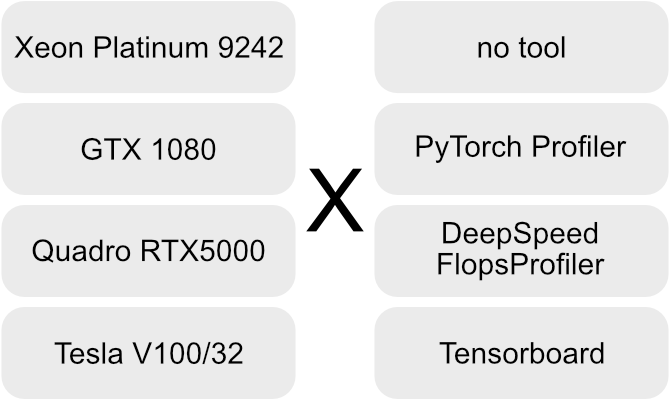
\includegraphics[width=0.9\textwidth]{../../data/experiments.png}
            \end{figure}
        \end{column}
        \begin{column}{0.5\textwidth}
            \begin{itemize}
                \item What is the benefit of using different accelerators?
                \item What is the cost for using profilers?
                \vspace{2em}
                \hline
                \vspace{2em}
                \item 4 different nodes of the SCC\footnote{\tiny{Scientific Compute Cluster}}\footnote{\tiny{\url{https://www.gwdg.de/web/guest/hpc-on-campus/scc}}, accessed on: 31.01.2023}
                \item 4 different tools
                \item[$\Rightarrow$] 16 runs
            \end{itemize}
            \vspace{1em}
        \end{column}
    \end{columns}

\end{frame}

\begin{frame}{Training setup}
\begin{itemize}
    \item number of trees for training: 8000 (740 GB)
    \vspace{1em}
    \item number of trees for testing: 2000 (191GB)
    \vspace{1em}
    \item trained for 15 epochs
\end{itemize}
\end{frame}


\begin{frame}{Long training times for original workflow}
    \begin{center}
    \begin{figure}
        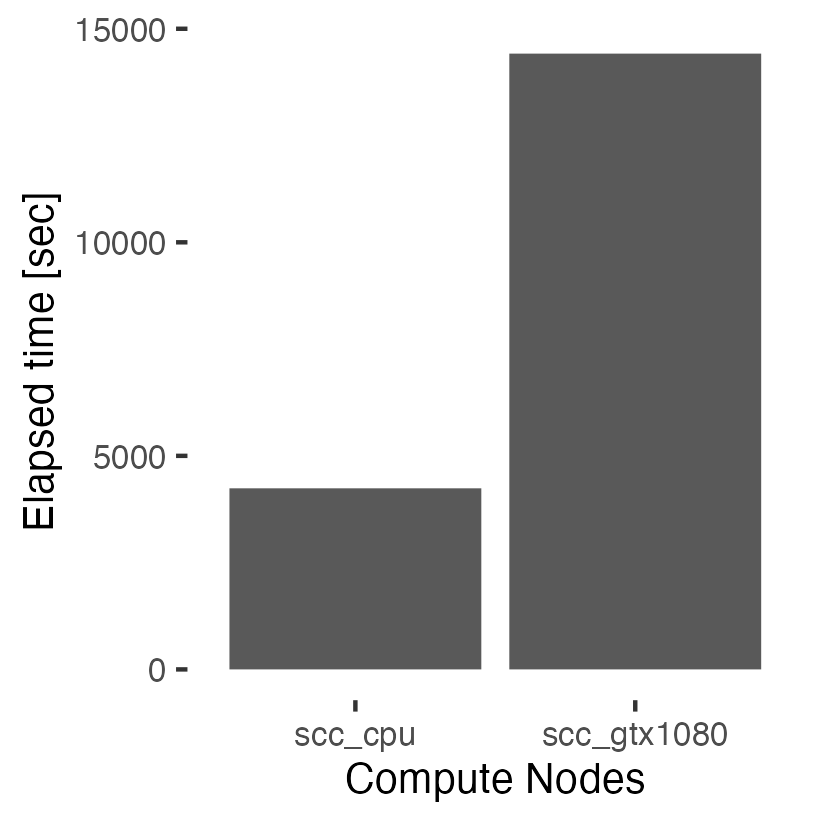
\includegraphics[width=0.5\textwidth]{../../data/sacct_barplot_by_nodes_profiler-torch_sample-points}
    \end{figure}
    \end{center}
\end{frame}

\begin{frame}{Trying to use the PyTorch Profiler to find the bottleneck}
	\vspace{-1em}
    \begin{center}
    \begin{figure}
        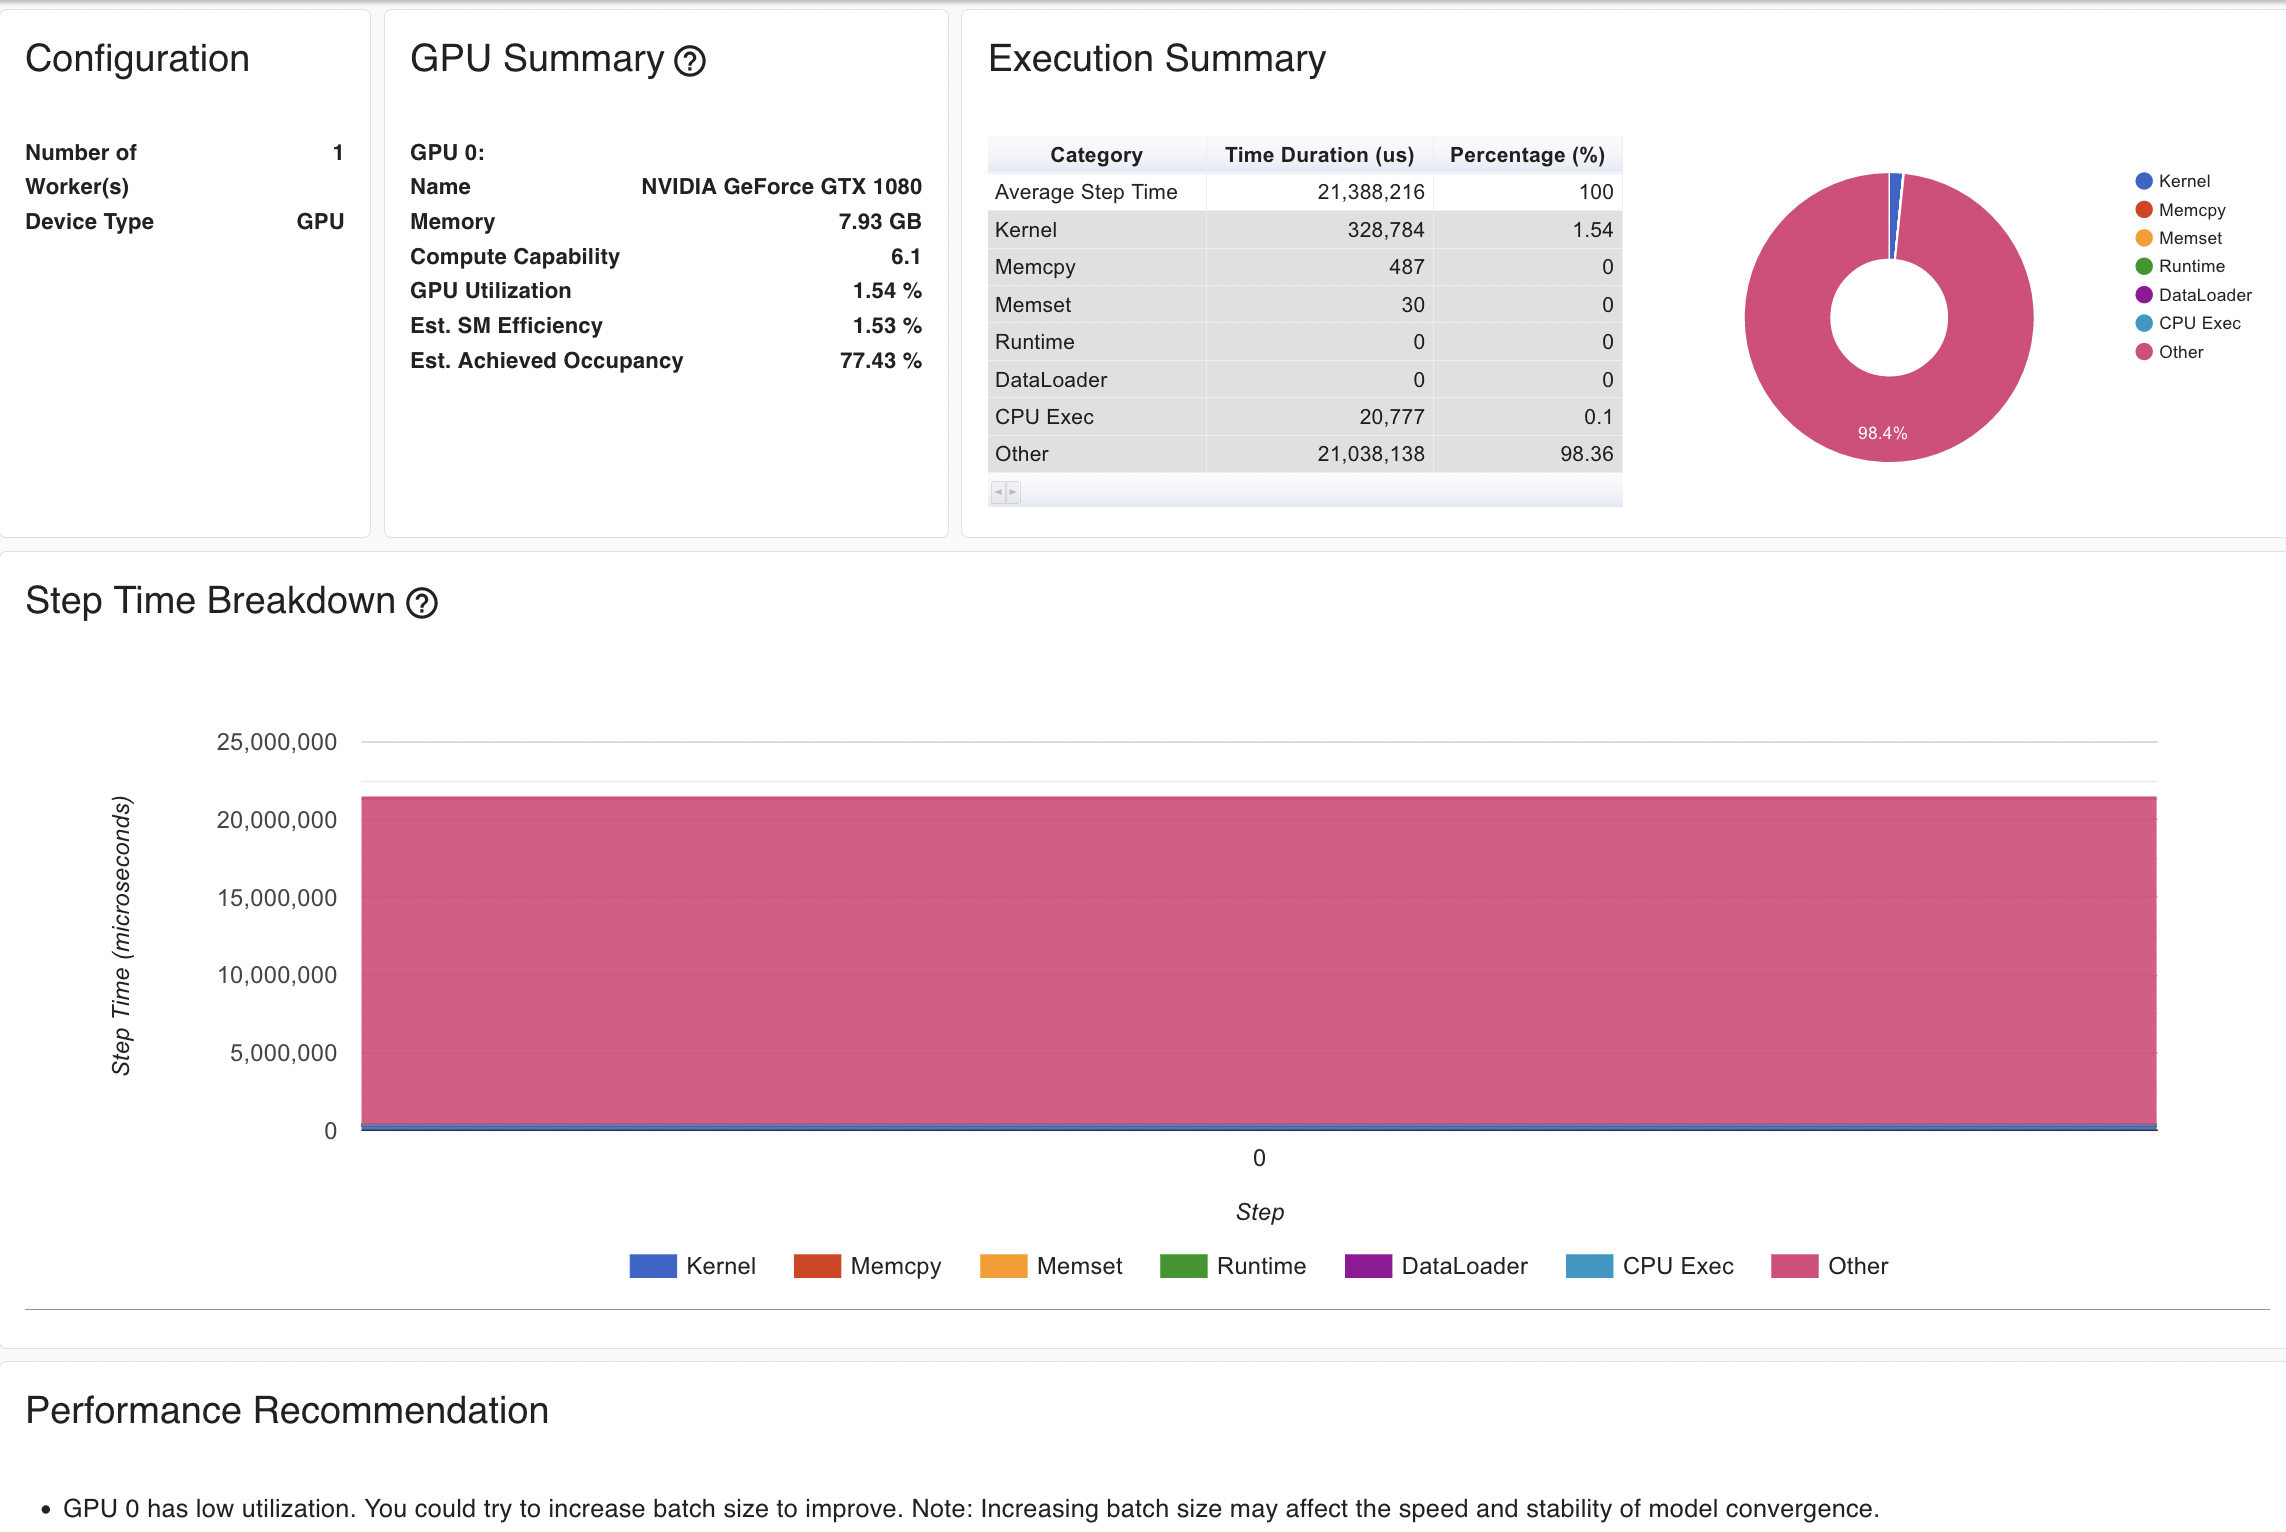
\includegraphics[width=0.75\textwidth]{../../data/scap_gtx1080_profiler-torch_sample-points_14650750}
    \end{figure}
    \end{center}
\end{frame}

\begin{frame}{Trying to use the PyTorch Profiler to find the bottleneck}
    \vspace{-1em}
    \begin{center}
    \begin{figure}
        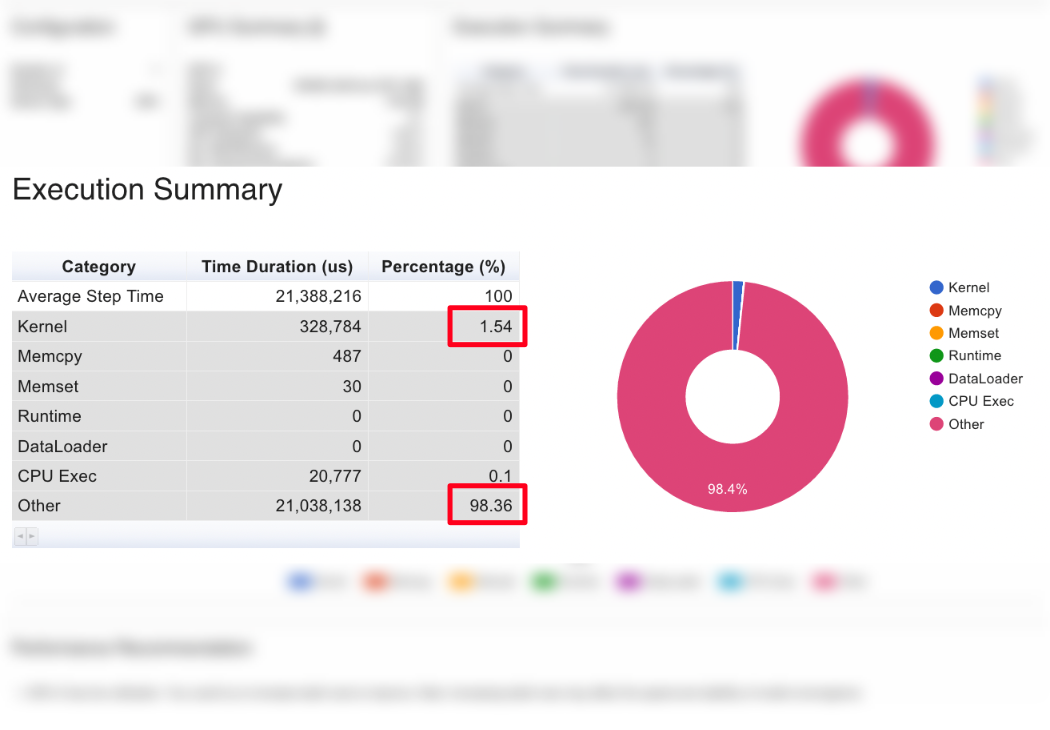
\includegraphics[width=0.9\textwidth]{../../data/scap_gtx1080_profiler-torch_sample-points_14650750_execution-time}
    \end{figure}
    \end{center}
\end{frame}

\begin{frame}{Identification of the bottleneck}

\begin{columns}
        \begin{column}{0.5\textwidth}
            \centering
            \vspace{-1em}
            \begin{figure}
            
\includegraphics[width=0.7\textwidth]{../../data/icon_question}
            \end{figure}
        \end{column}
        \begin{column}{0.5\textwidth}
            \begin{itemize}
                \item bottleneck
                \begin{itemize}
                    \item data loading and \\sampling process
                \end{itemize}
                \item solution
                    \begin{itemize}
                        \item sample points before training
                    \end{itemize}
                \vspace{2em}
                \hline
                \vspace{2em}
                \item without help of the PyTorch Profiler
            \end{itemize}
        \end{column}
    \end{columns}

\end{frame}

\begin{frame}{Effect of point sampling strategies on walltime}
    \vspace{-1em}
    \begin{center}
    \begin{figure}
        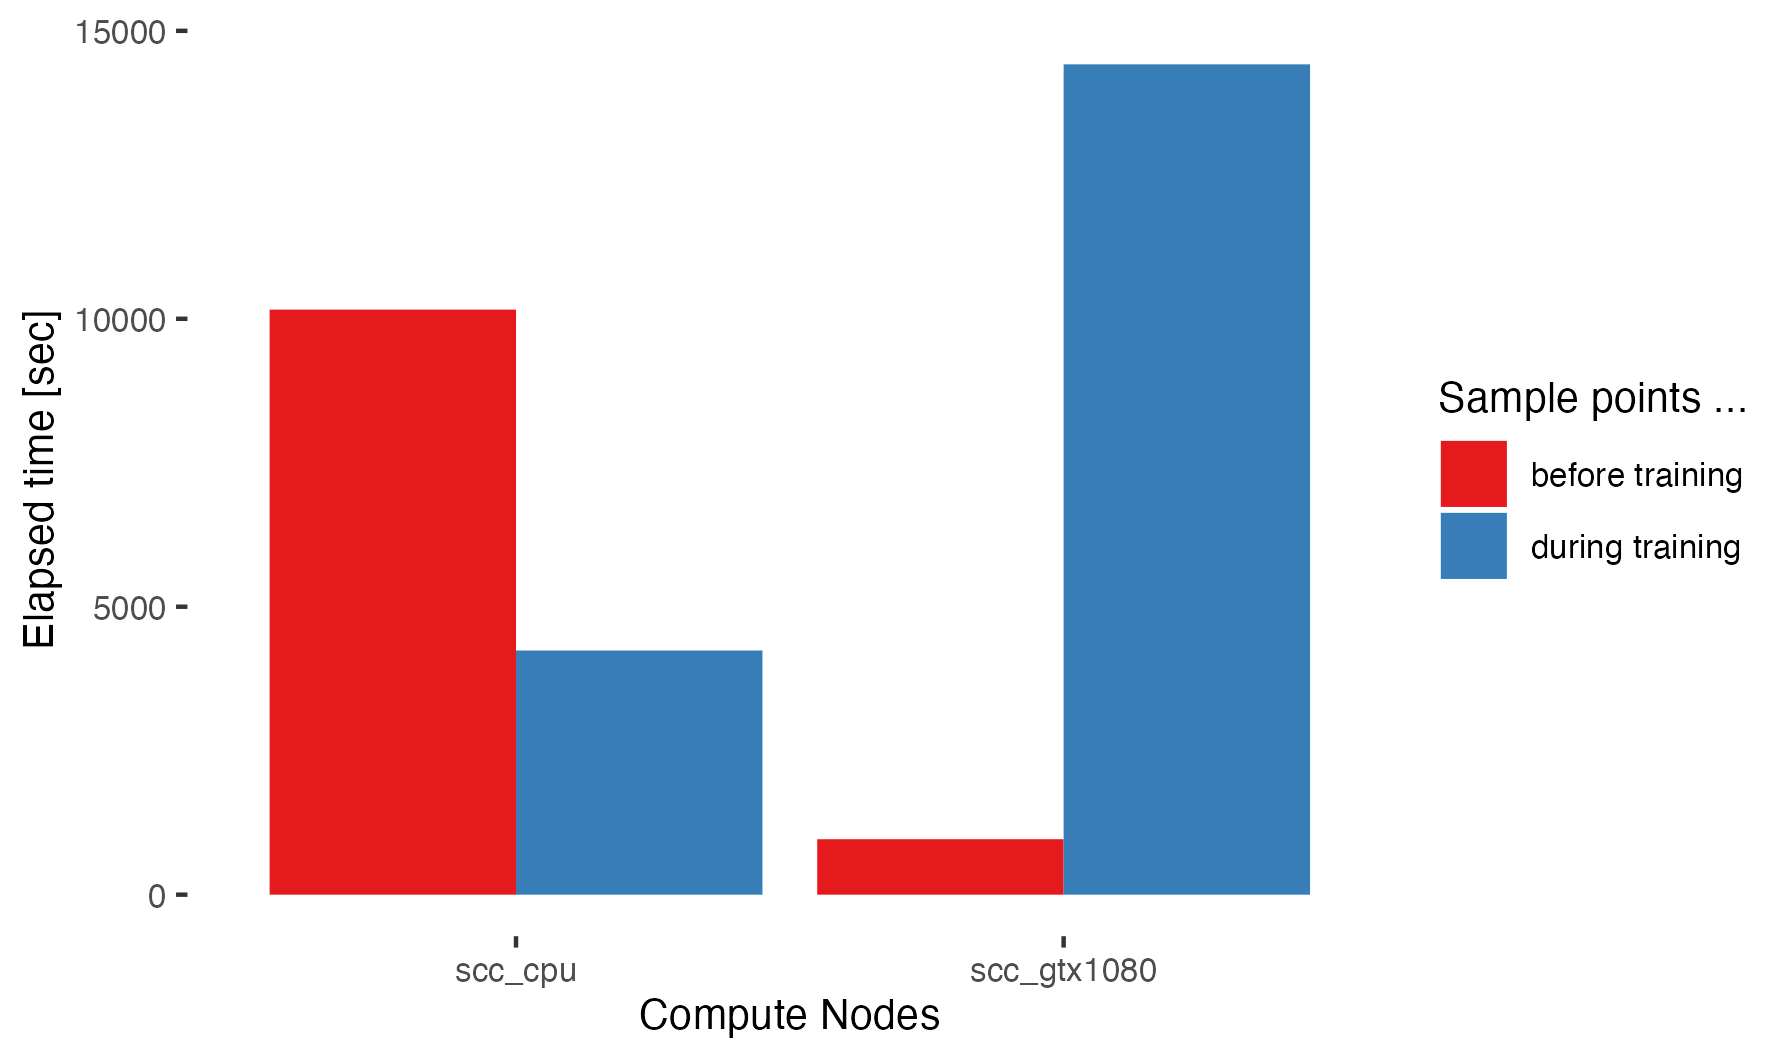
\includegraphics[width=0.85\textwidth]{../../data/sacct_barplot_by_nodes_sample-points-effect}
    \end{figure}
    \end{center}
\end{frame}

\begin{frame}{Training setup - improved}
\begin{itemize}
    \item number of trees for training: 8000 (\sout{740 GB} 434 MB)
    \vspace{1em}
    \item number of trees for testing: 2000 (\sout{191 GB} 109MB)
    \vspace{1em}
    \item trained for 15 epochs
    \vspace{2em}
    \hline
    \vspace{2em}
    \item[$\rightarrow$] reduced hardware usage (energy + money savings)
    \item[$\rightarrow$] more variations of hardware and tools can be tested
\end{itemize}
\end{frame}

\begin{frame}{Tabular overview}
% Please add the following required packages to your document preamble:
% \usepackage{booktabs}
\scriptsize{
% Please add the following required packages to your document preamble:
% \usepackage{booktabs}
\begin{table}[]
\begin{tabular}{@{}llllll@{}}
\toprule
run & node         & tool           & job\_id  & is\_valid  \\ \midrule
1   & scc\_cpu     & no-tool        & 14629421 & TRUE                  \\
2   & scc\_cpu     & tensorboard    & 14629426 & TRUE                  \\
3   & scc\_cpu     & profiler-torch & 14650740 & TRUE                  \\
4   & scc\_cpu     & deepspeed      & 14617521 & FALSE                 \\
5   & scc\_gtx1080 & no-tool        & 14619617 & TRUE                  \\
6   & scc\_gtx1080 & tensorboard    & 14615343 & TRUE                  \\
7   & scc\_gtx1080 & profiler-torch & 14650076 & TRUE                  \\
8   & scc\_gtx1080 & deepspeed      & 14615344 & TRUE                  \\
9   & scc\_rtx5000 & no-tool        & 14619618 & TRUE                  \\
10  & scc\_rtx5000 & tensorboard    & 14617172 & TRUE                  \\
11  & scc\_rtx5000 & profiler-torch & 14650079 & TRUE                  \\
12  & scc\_rtx5000 & deepspeed      & 14617171 & TRUE                  \\
13  & scc\_v100    & no-tool        & 14619619 & TRUE                  \\
14  & scc\_v100    & tensorboard    & 14617203 & TRUE                  \\
15  & scc\_v100    & profiler-torch & 14650080 & TRUE                  \\
16  & scc\_v100    & deepspeed      & 14617202 & TRUE                 
\end{tabular}
\end{table}
}
\end{frame}

\begin{frame}{Runtime on HPC}
    \begin{center}
    \begin{figure}
        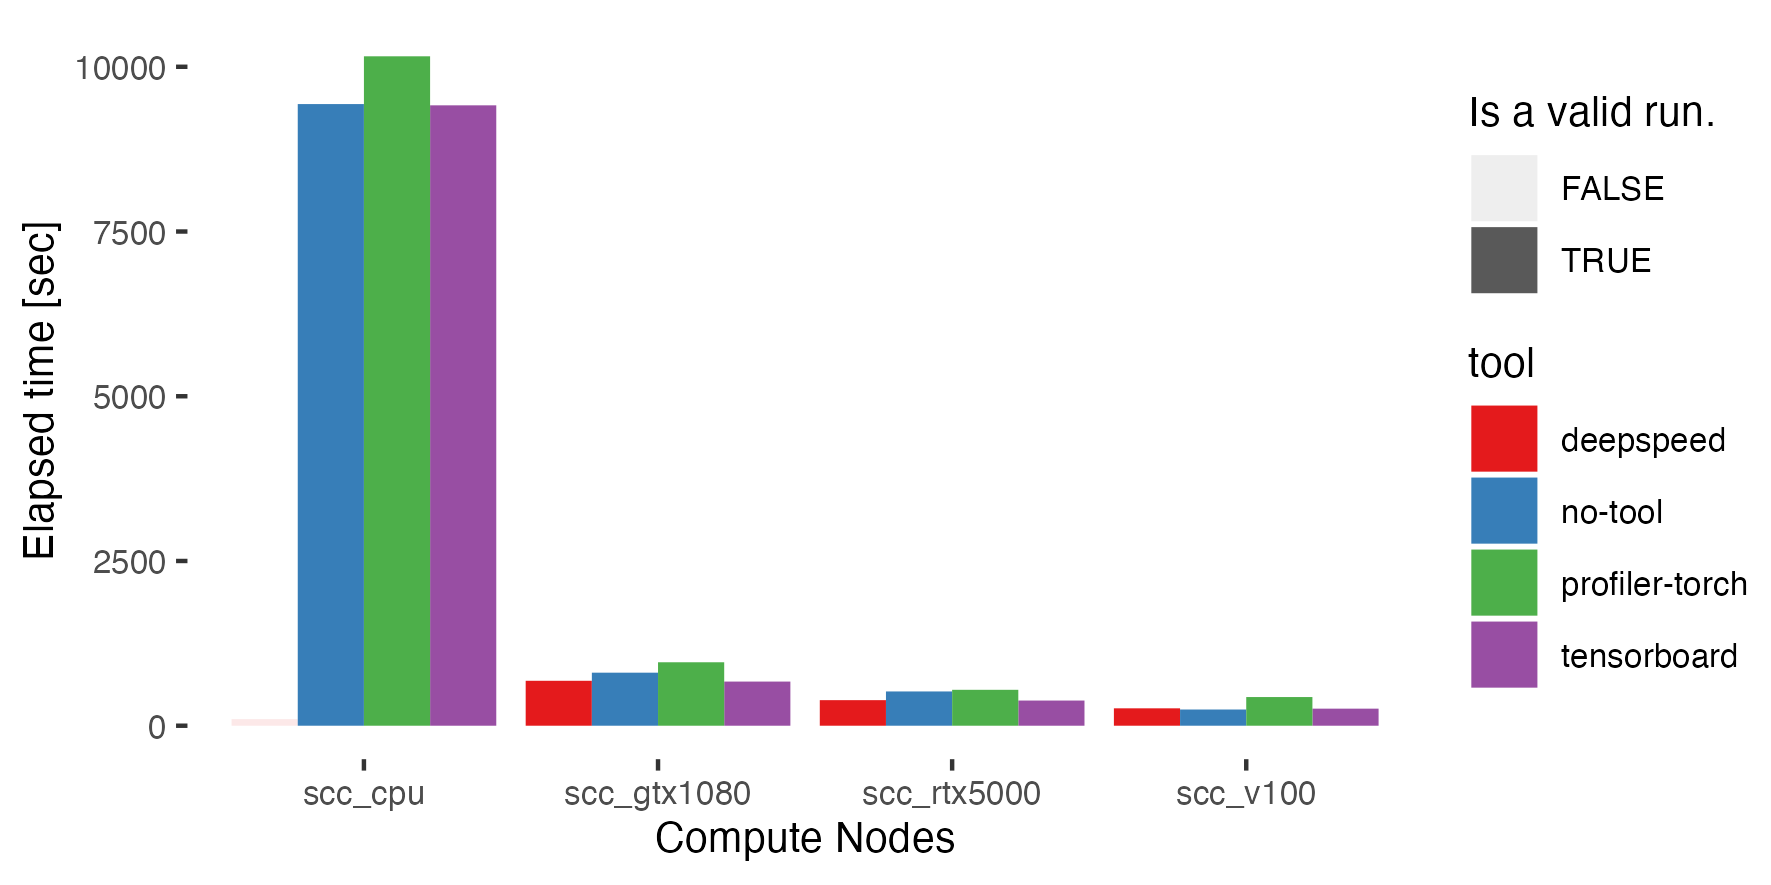
\includegraphics[width=1\textwidth]{../../data/sacct_barplot_by_nodes_no-experiment}
    \end{figure}
    \end{center}
\end{frame}

\begin{frame}{Runtime on HPC (GPU-only)}
    \begin{center}
    \begin{figure}
        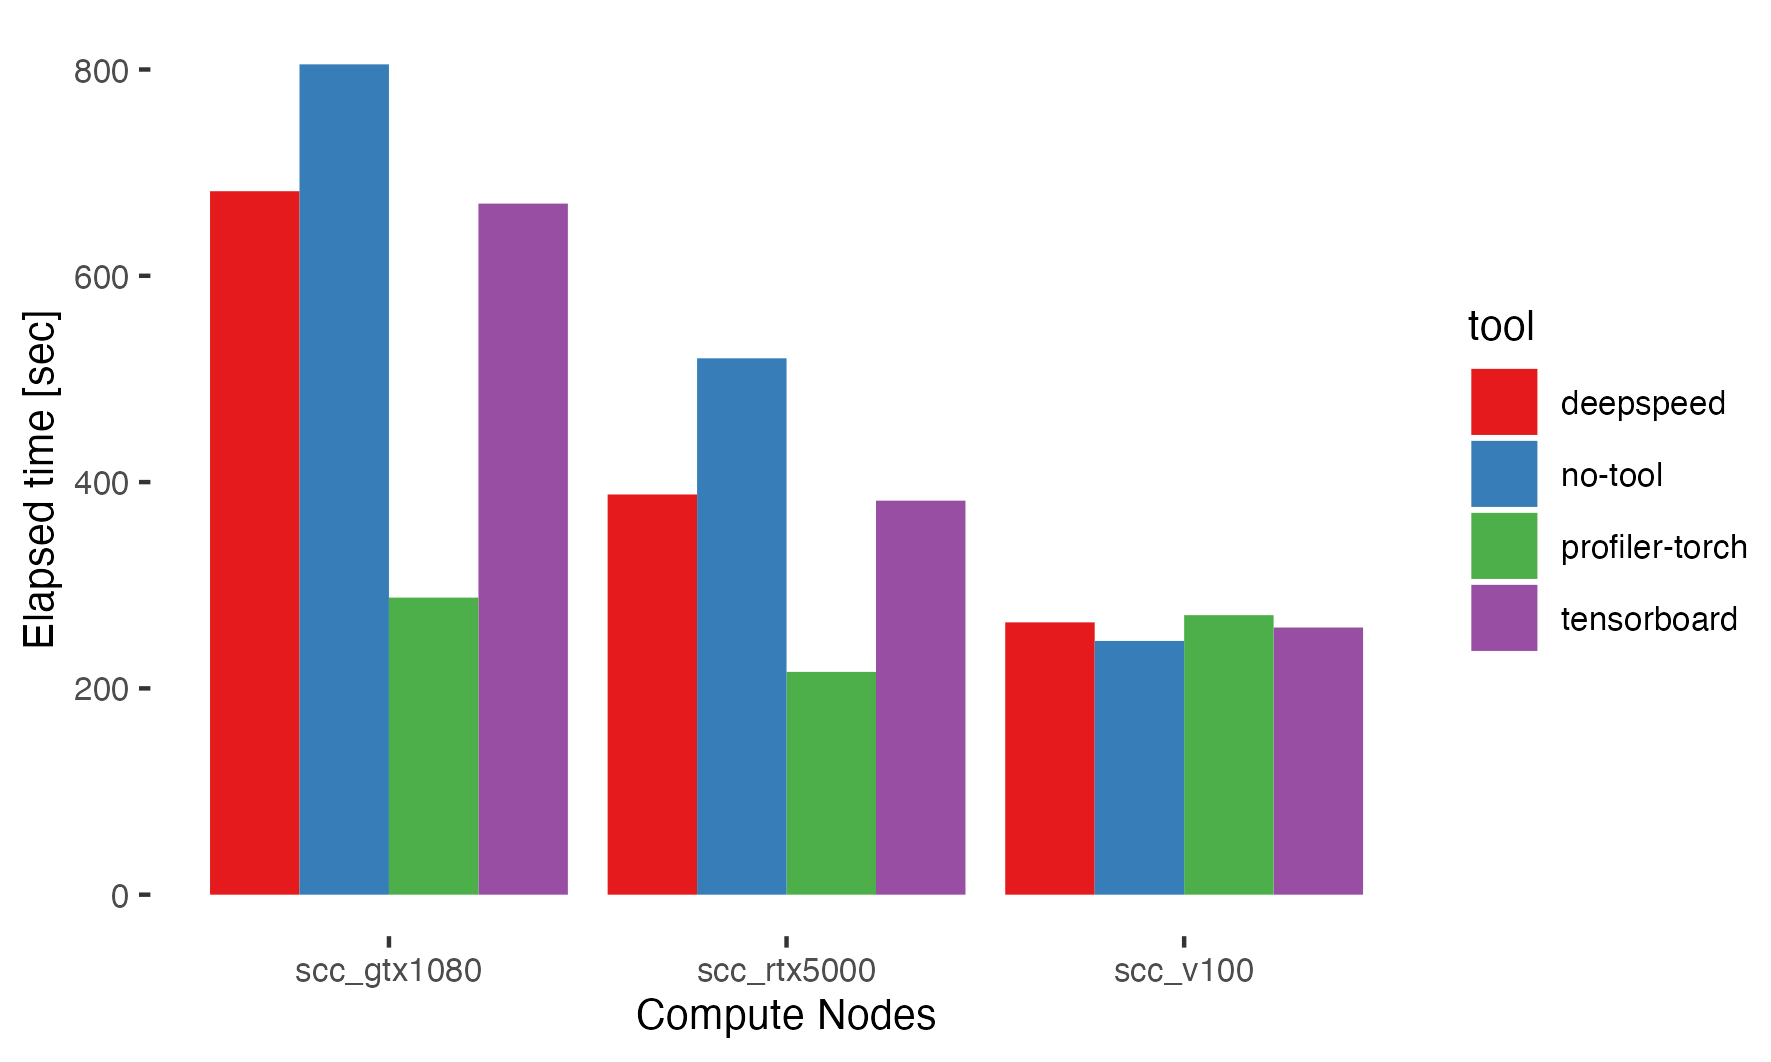
\includegraphics[width=0.87\textwidth]{../../data/sacct_barplot_by_nodes_no-experiment_gpu}
    \end{figure}
    \end{center}
\end{frame}

\begin{frame}[fragile]{So far we just analyzed the wall time}
\footnotetext[1]{test}
\begin{columns}
\begin{column}{0.7\textwidth}
        \begin{minted}[breaklines, fontsize=\scriptsize ]{python}
sacct --format=jobid,elapsed -P -j 14657599, 14617521, 14615343, 14650076, 14615344, 14617172, 14650079, 14617171, 14618941, 14617203, 14619619, 14650080, 14619618,14619617, 14617202, 14650750, 14650758, 14629421, 14629426, 14650740, 14650759 -X
        \end{minted}
\end{column}

\begin{column}{0.3\textwidth}
    \vspace{-2em}
        \inputminted[xleftmargin=1em,linenos,fontsize=\tiny,]{python}{../../data/sacct.out}
\end{column}
\end{columns}
\end{frame}

\section{PyTorch Profiler}
%\sectionIntroHidden % Show an outline of the current section with hidden subsections
\sectionIntro % Show an outline of the current section with subsections

\begin{frame}{PyTorch Profiler: Views}
\begin{itemize}
    \item \textbf{Overview}
    \item Operator View
    \item GPU Kernel View
    \item \textbf{Trace View}
    \item Memory View
    \item Module View
\end{itemize}
\end{frame}

\begin{frame}{Overview}
	\vspace{-1em}
\begin{center}
    \begin{figure}
        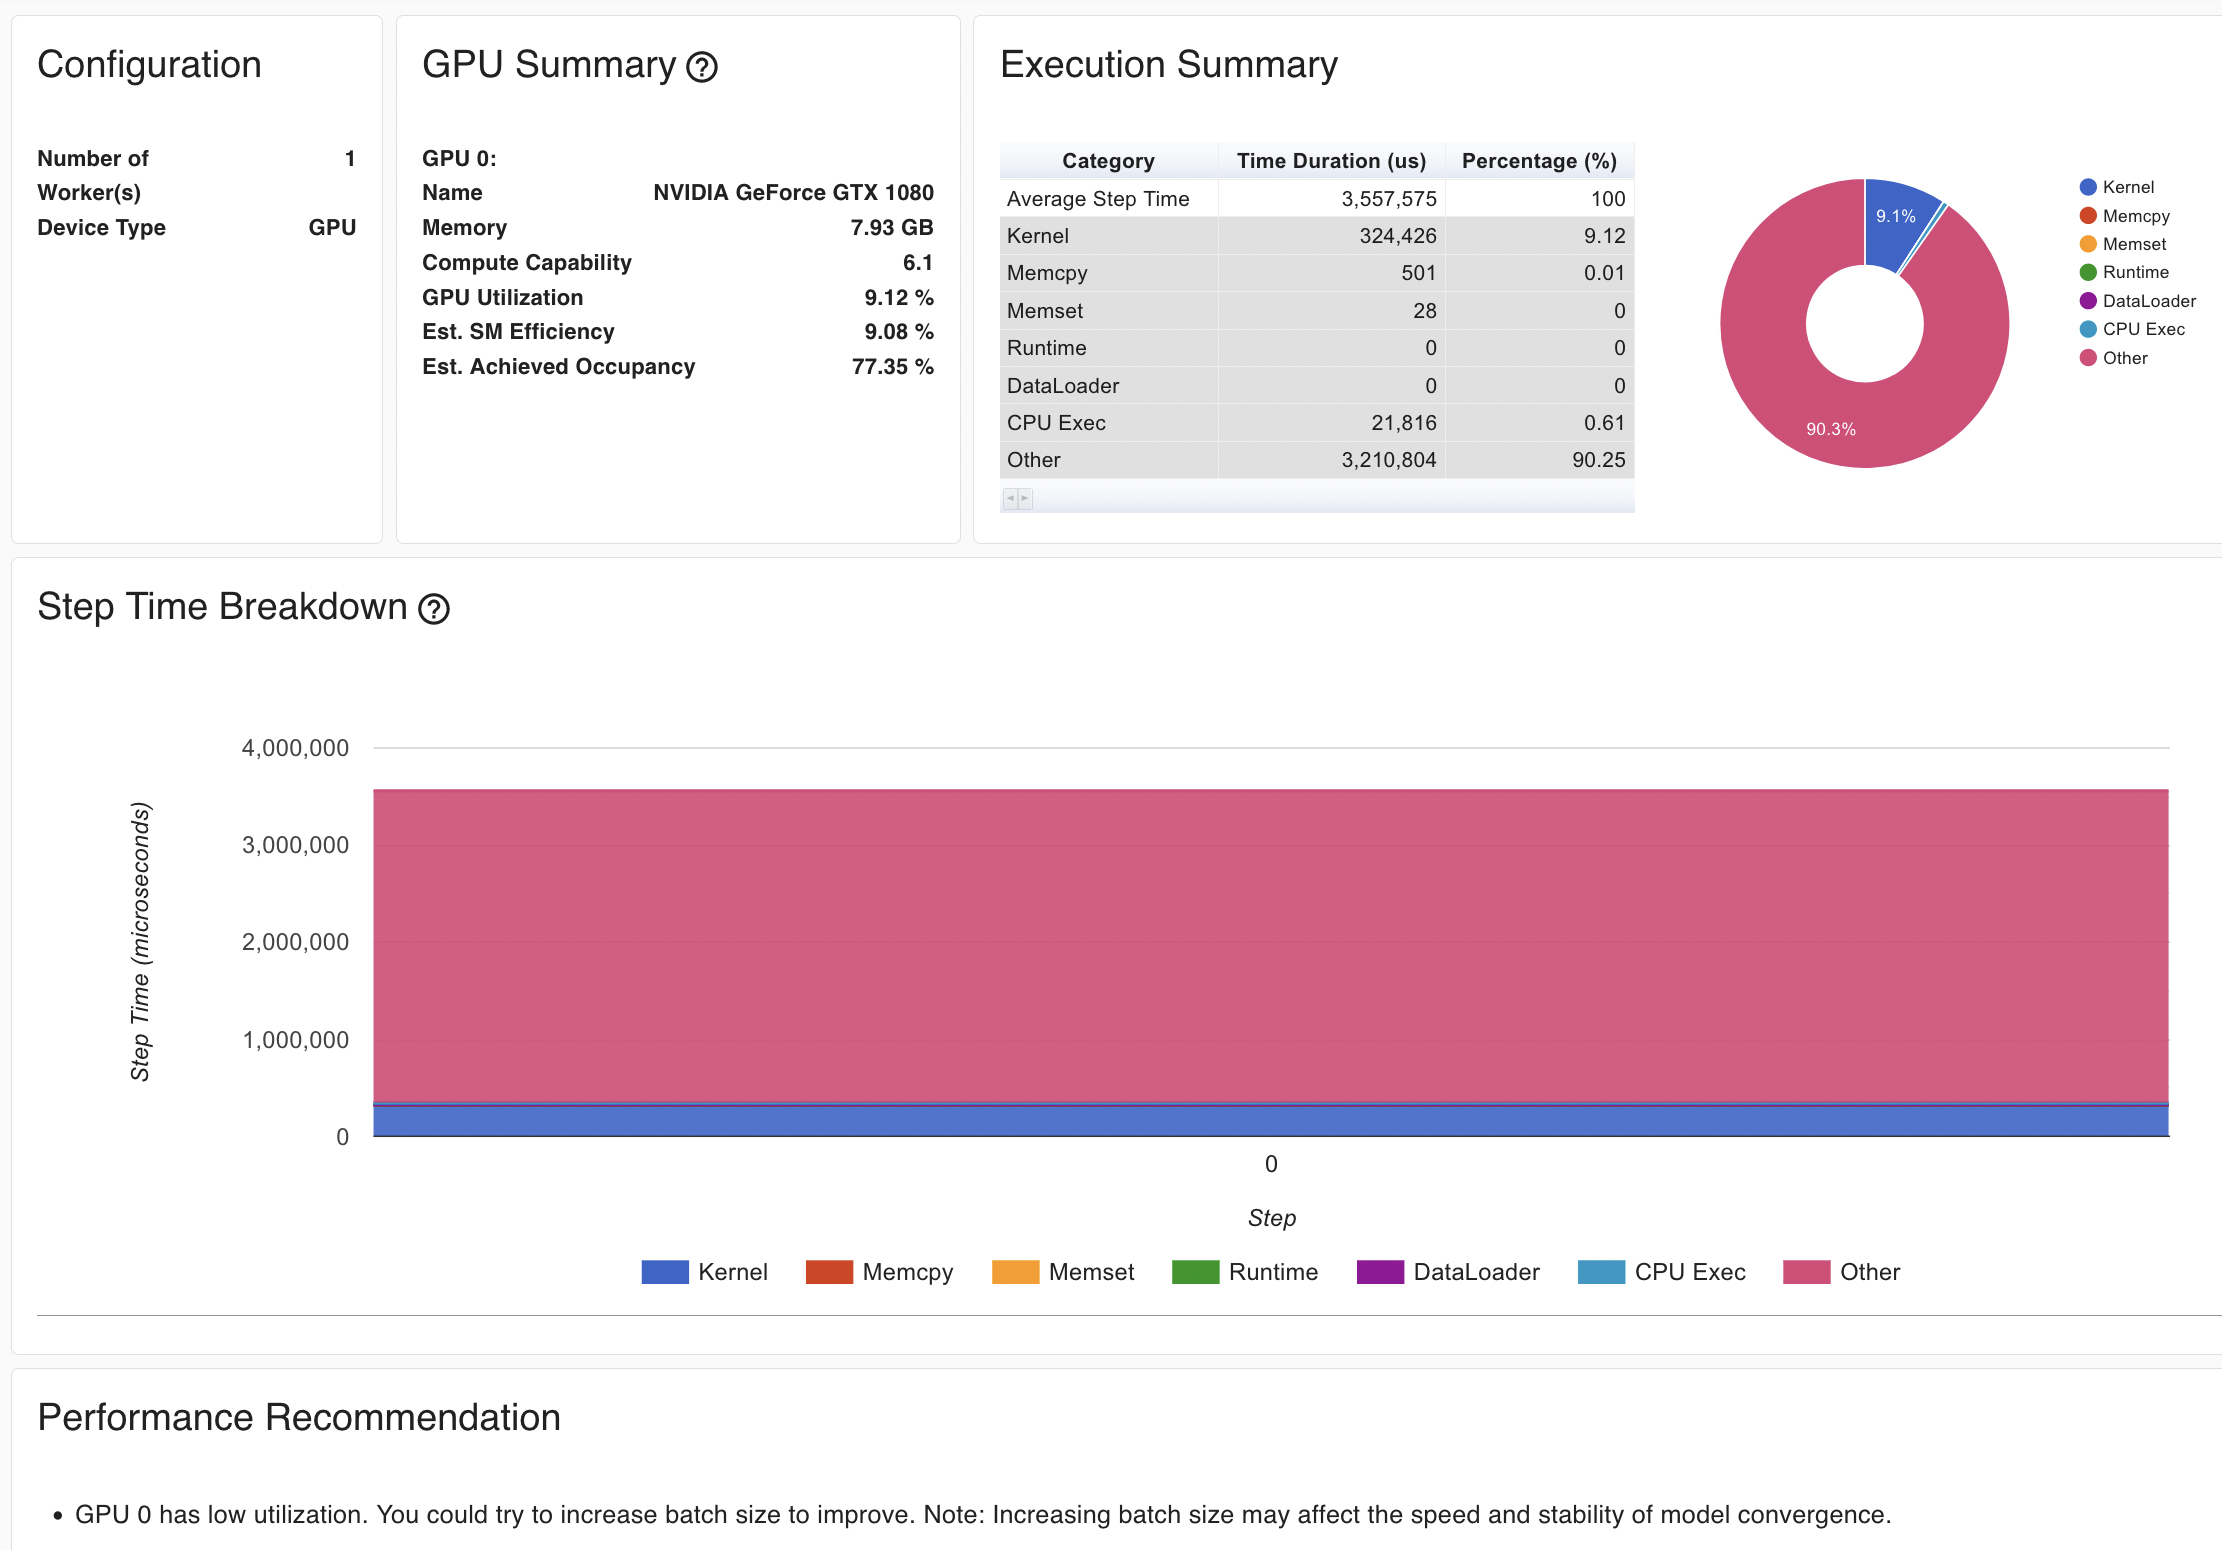
\includegraphics[width=0.7\textwidth]{../../data/scap_gtx1080_profiler-torch_14650076}
    \end{figure}
\end{center}

\end{frame}

\begin{frame}{Performance Recommendation}

\begin{center}
    \begin{figure}
        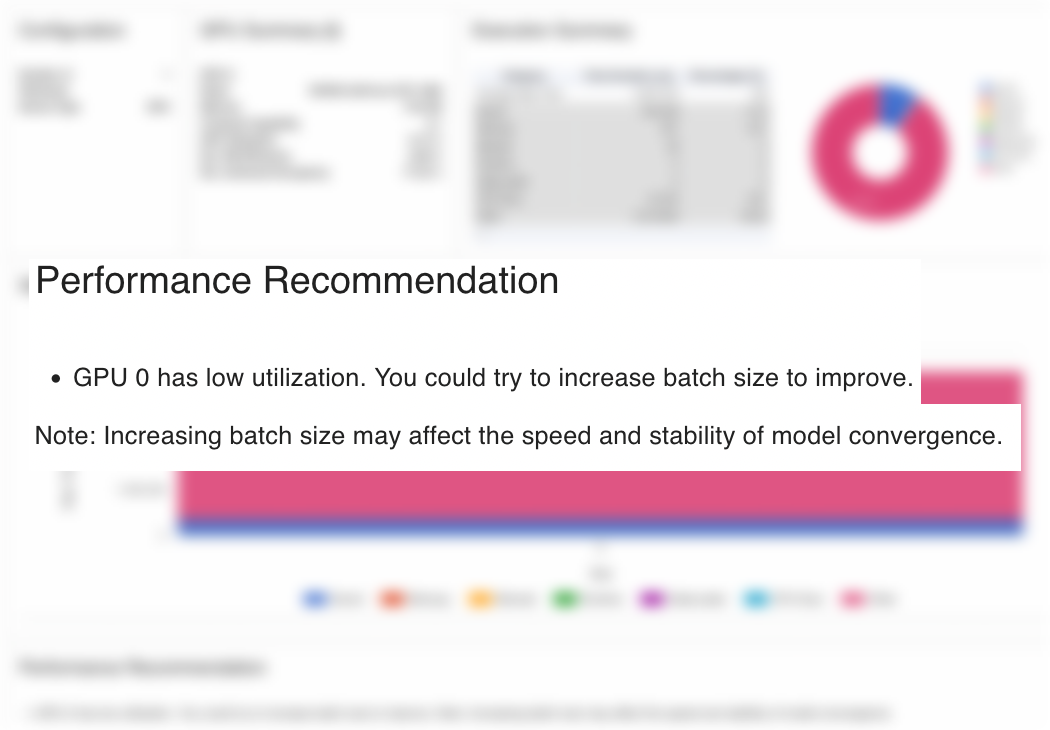
\includegraphics[width=0.7\textwidth]{../../data/scap_gtx1080_profiler-torch_14650076_zoom}
    \end{figure}
\end{center}

\end{frame}


\begin{frame}{Effect of increasing the batch size}
    \vspace{-0.5em}
\begin{center}
    \begin{figure}
        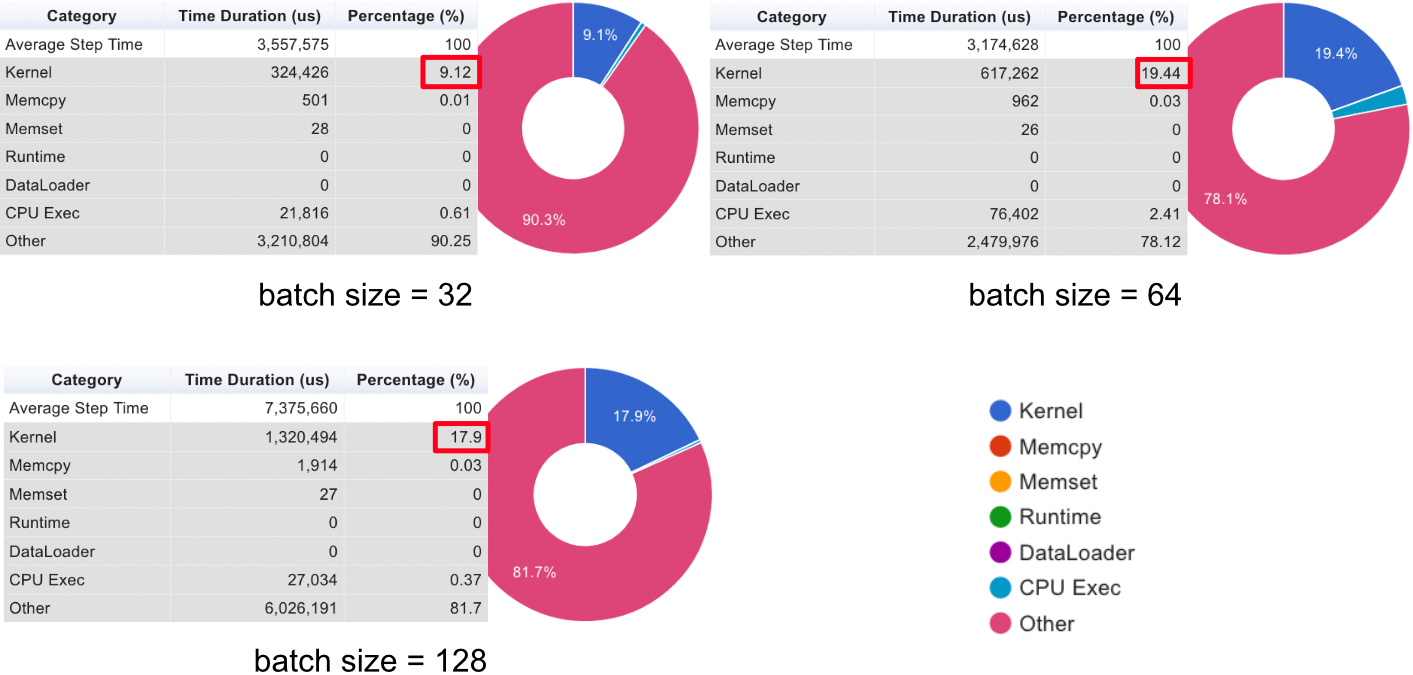
\includegraphics[width=1\textwidth]{../../data/scap_gtx1080_profiler-torch_comparison-batch-size}
    \end{figure}
    \end{center}

\end{frame}

\begin{frame}{Trace View}
    \vspace{-1em}
\begin{center}
    \begin{figure}
        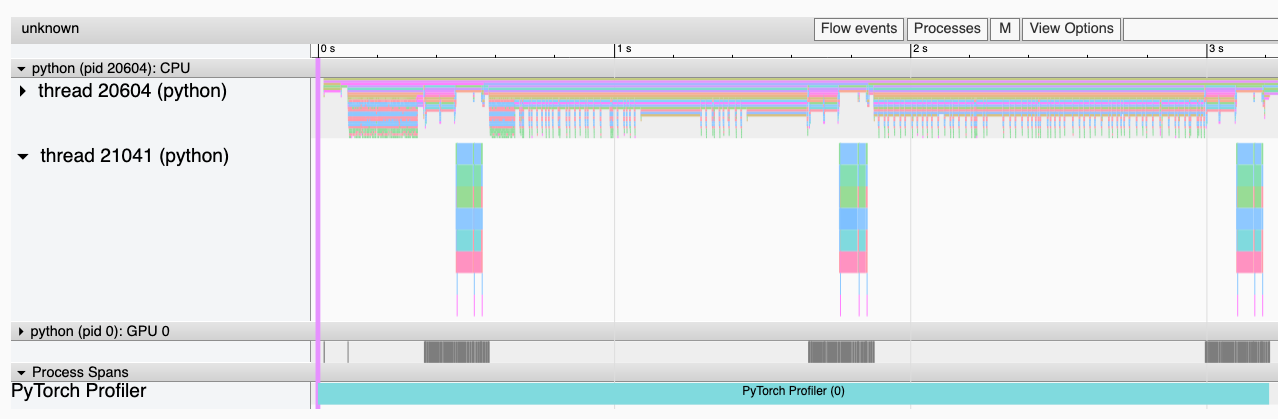
\includegraphics[width=1\textwidth]{../../data/scap_gtx1080_profiler-torch_batch-size-64_14650758_trace-view}
    \end{figure}
    \end{center}
\end{frame}

\begin{frame}{Trace View: Laspy with presampled lidar data}
    \vspace{-1em}
\begin{center}
    \begin{figure}
        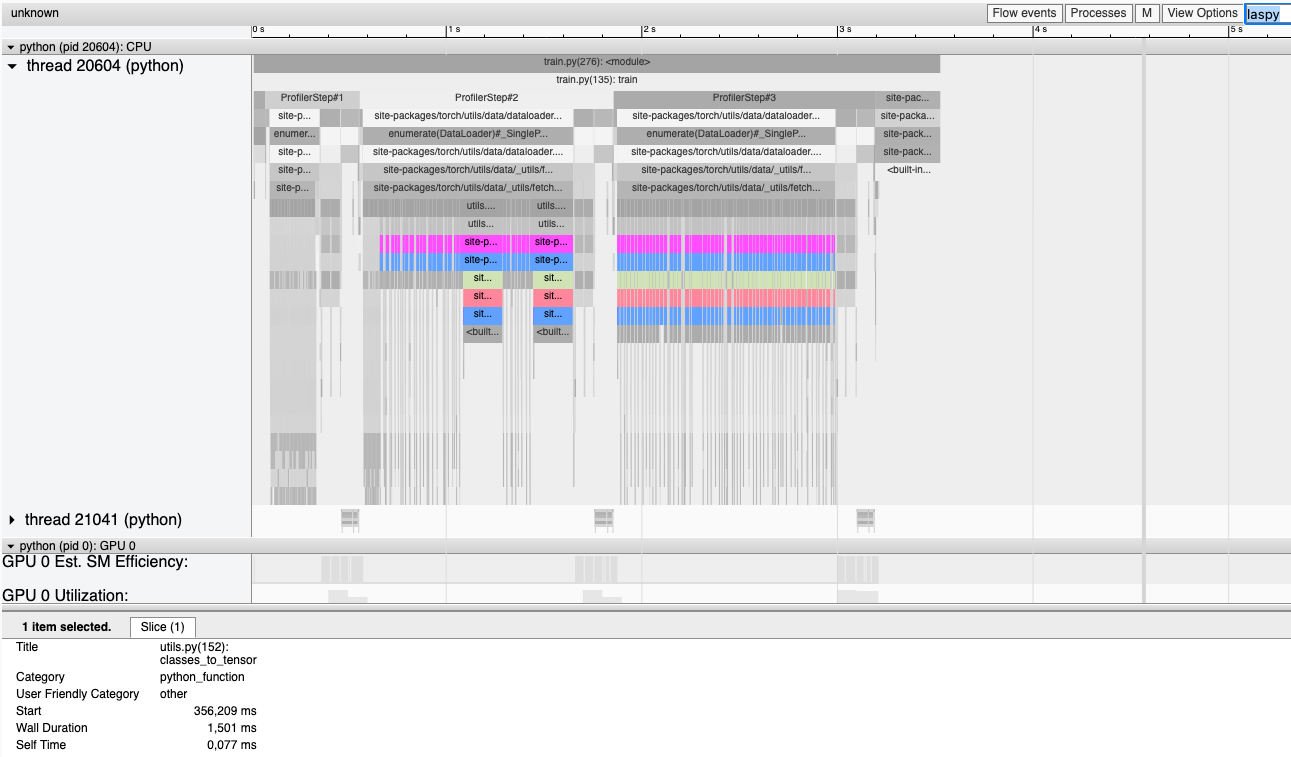
\includegraphics[width=1\textwidth]{../../data/scap_gtx1080_profiler-torch_batch-size-64_14650758_trace-view-laspy}
    \end{figure}
    \end{center}
\end{frame}

\begin{frame}{Trace View: Laspy with raw lidar data}
    \vspace{-1em}
\begin{center}
    \begin{figure}
        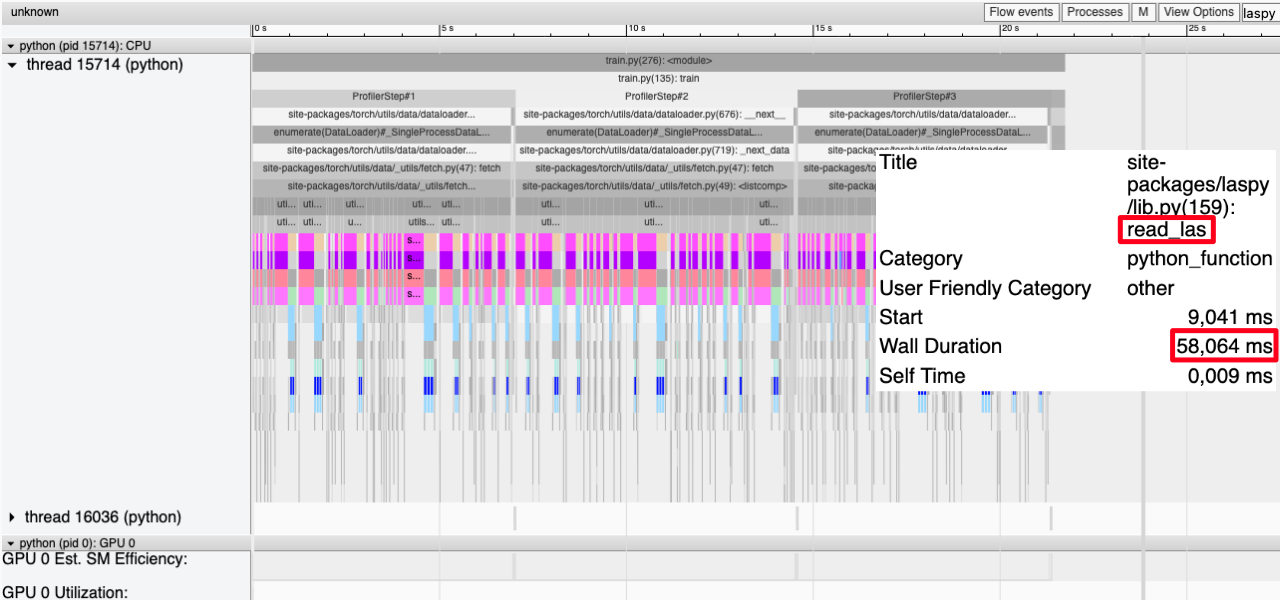
\includegraphics[width=1\textwidth]{../../data/scap_gtx1080_profiler-torch_sample-points_14650750_trace-view-laspy}
    \end{figure}
    \end{center}
\end{frame}

%%%%%%%%%%%%%%%%

\section{Deepspeed - FlopsProfiler}
%\sectionIntroHidden % Show an outline of the current section with hidden subsections
\sectionIntro % Show an outline of the current section with subsections

\begin{frame}[fragile]{Summary}
        \footnotesize\inputminted[xleftmargin=1em,linenos,fontsize=\scriptsize, firstline=1,lastline=16]{python}{../../data/scap_gtx1080_deepspeed_14615344_4294967294_one-epoch.txt}

\end{frame}

\begin{frame}[fragile]{Aggregated Profile per GPU}
        \footnotesize\inputminted[xleftmargin=1em,linenos,fontsize=\scriptsize, firstline=18,lastline=31]{python}{../../data/scap_gtx1080_deepspeed_14615344_4294967294_one-epoch.txt}

\end{frame}

\begin{frame}[fragile]{Detailed Profile per GPU}
        \footnotesize\inputminted[xleftmargin=1em,linenos,fontsize=\tiny, firstline=33,lastline=48, breaklines]{python}{../../data/scap_gtx1080_deepspeed_14615344_4294967294_one-epoch.txt}

\end{frame}




\section{Conclusion}
%\sectionIntroHidden % Show an outline of the current section with hidden subsections
\sectionIntro % Show an outline of the current section with subsections

\begin{frame}{Conclusion}
\begin{itemize}
    \item[$\checkmark$] Identification of profiling tools
    \begin{itemize}
        \item[\textcolor{c3}{\textbullet}] \textbf{PyTorch Profiler}: similar to "typical" software profilers
        \item[\textcolor{c5}{\textbullet}] \textbf{FlopsProfiler}: more intuitive from a deep learning perspective
        \item[\textcolor{c5}{\textbullet}] most important metrics are available
        \item[$\rightarrow$] Combination of both is most promising
    \end{itemize}
    \vspace{1cm}
    \item[($\checkmark$)] Usability
    \begin{itemize}
        \item[\textcolor{c3}{\textbullet}] easy to setup
        \item[\textcolor{c3}{\textbullet}] some low hanging fruits (e.g. performance recommendations)
        \item[\textcolor{c1}{\textbullet}] generally a deep dive into the code and the network architecture is required
    \end{itemize}
\end{itemize}
\end{frame}

\begin{frame}{Try it yourself!}
\label{pg:lastpage} % Label on last frame to get the page number for footer

\begin{columns}
        \begin{column}{0.45\textwidth}
            \centering
            \vspace{-1em}
            \begin{figure}
            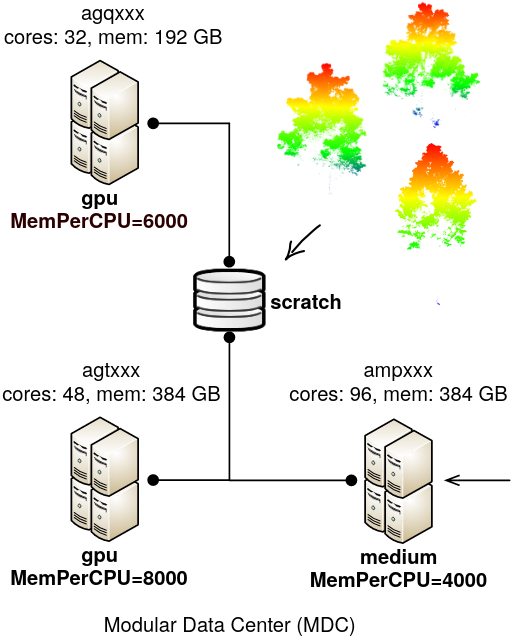
\includegraphics[width=0.7\textwidth]{../../data/gwdg_scc_tree-data}
            \caption*{Synthetic lidar data is available on the SCC.}
            \end{figure}
        \end{column}
        \begin{column}{0.55\textwidth}
            \begin{itemize}
                \item data is on scratch of the SCC\footnote{\tiny{\texttt{/scratch/projects/workshops/forest/synthetic\_trees\_ten\_sampled}}}
                \vspace{1em}
                \item code for this course is available \\on Github\footnote{\tiny{\url{https://github.com/haukekirchner/scap/}}}
                \vspace{1em}
                \item additional read:\\workshop Forests in HPC\footnote{\tiny{\url{https://gitlab-ce.gwdg.de/hauke.gronenberg/workshop-forests-in-hpc}}}
                \vspace{1em}
            \end{itemize}
        \end{column}
    \end{columns}

\source{Image source: Adapted from \url{https://www.gwdg.de/web/guest/hpc-on-campus/scc}, accessed on: 09.11.2022}

\end{frame}

\appendix
\backupbegin

\begin{frame}{References}
    % References slide in appendix
    \renewcommand*{\bibfont}{\normalfont\scriptsize}
    \printbibliography[heading=none]
\end{frame}

\begin{frame}{All runs}
% Please add the following required packages to your document preamble:
% \usepackage{booktabs}
\tiny{
% Please add the following required packages to your document preamble:
% \usepackage{booktabs}
\begin{table}[]
\begin{tabular}{@{}llllll@{}}
\toprule
run & node         & tool           & job\_id  & is\_valid & experiment     \\ \midrule
1   & scc\_cpu     & no-tool        & 14629421 & TRUE      &                \\
2   & scc\_cpu     & tensorboard    & 14629426 & TRUE      &                \\
3   & scc\_cpu     & profiler-torch & 14650740 & TRUE      &                \\
4   & scc\_cpu     & deepspeed      & 14617521 & FALSE     &                \\
5   & scc\_gtx1080 & no-tool        & 14619617 & TRUE      &                \\
6   & scc\_gtx1080 & tensorboard    & 14615343 & TRUE      &                \\
7   & scc\_gtx1080 & profiler-torch & 14650076 & TRUE      &                \\
8   & scc\_gtx1080 & deepspeed      & 14615344 & TRUE      &                \\
9   & scc\_rtx5000 & no-tool        & 14619618 & TRUE      &                \\
10  & scc\_rtx5000 & tensorboard    & 14617172 & TRUE      &                \\
11  & scc\_rtx5000 & profiler-torch & 14650079 & TRUE      &                \\
12  & scc\_rtx5000 & deepspeed      & 14617171 & TRUE      &                \\
13  & scc\_v100    & no-tool        & 14619619 & TRUE      &                \\
14  & scc\_v100    & tensorboard    & 14617203 & TRUE      &                \\
15  & scc\_v100    & profiler-torch & 14650080 & TRUE      &                \\
16  & scc\_v100    & deepspeed      & 14617202 & TRUE      &                \\
17  & scc\_gtx1080 & profiler-torch & 14650758 & TRUE      & batch-size-64  \\
18  & scc\_gtx1080 & profiler-torch & 14650750 & TRUE      & sample-points  \\
19  & scc\_cpu     & profiler-torch & 14657599 & TRUE      & sample-points  \\
20  & scc\_gtx1080 & profiler-torch & 14650759 & TRUE      & batch-size-128 \\ \bottomrule
\end{tabular}
\end{table}
}
\end{frame}

\begin{frame}{Tensorboard for run with GTX1080}

\begin{center}
    \begin{figure}
        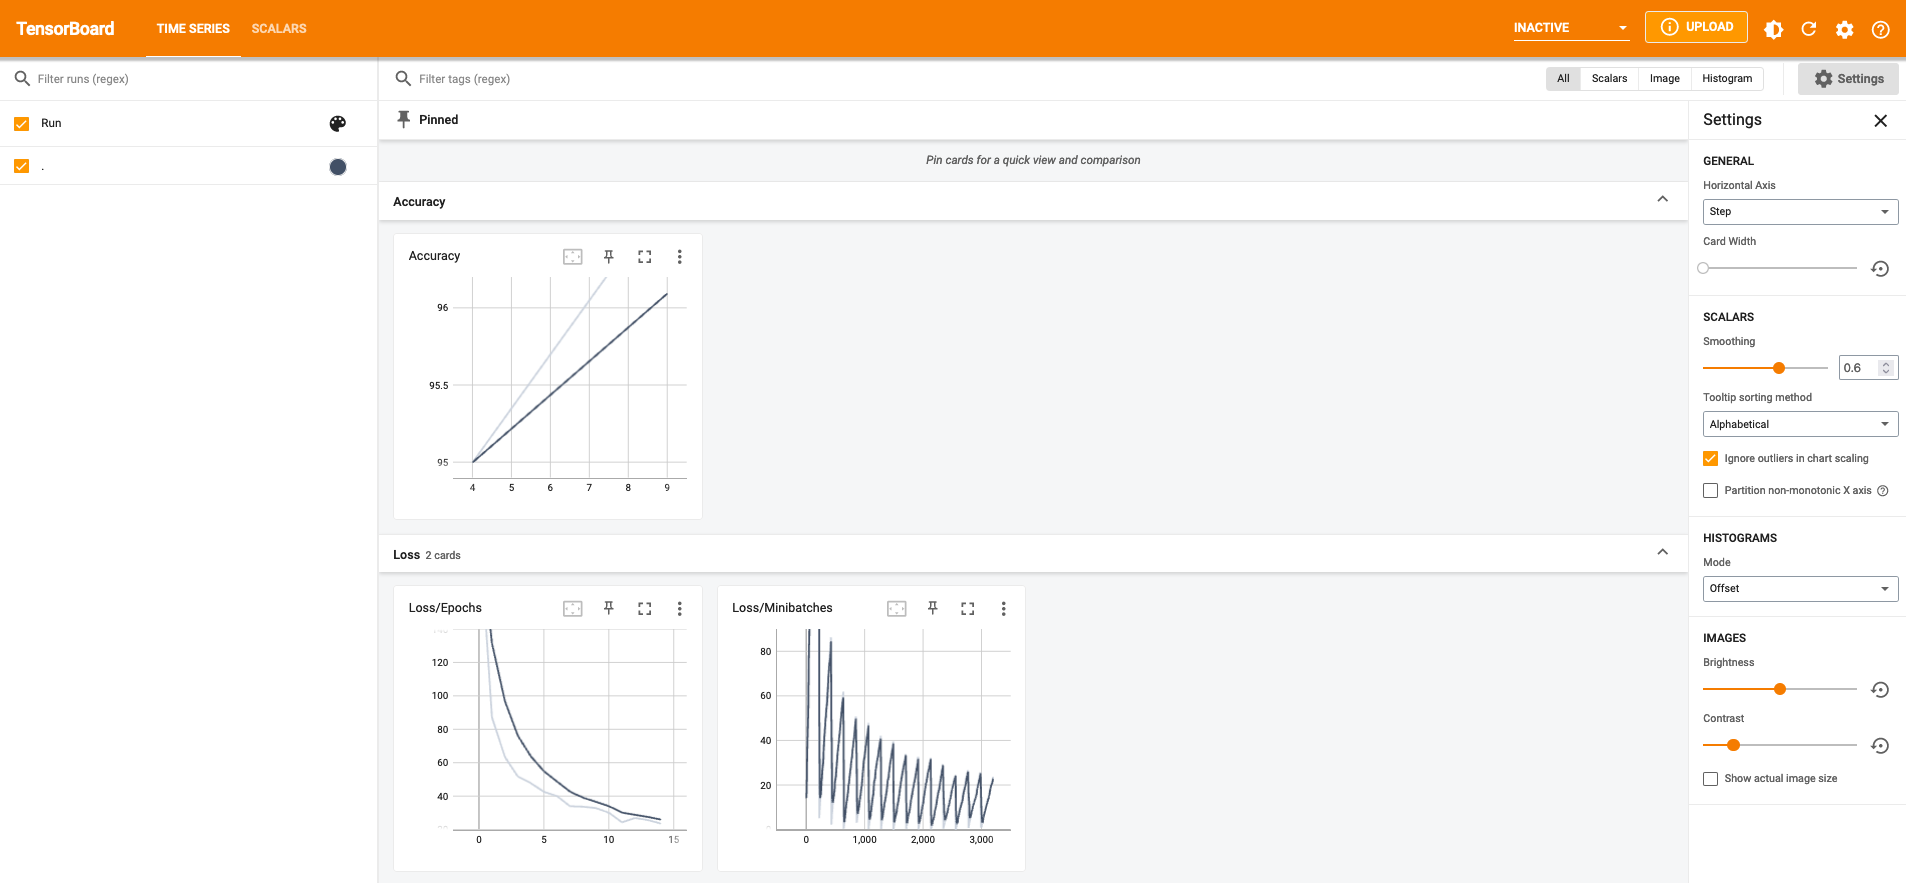
\includegraphics[width=1\textwidth]{../../data/scap_gtx1080_tensorboard_14615343}
    \end{figure}
    \end{center}

\end{frame}

\begin{frame}{result of increasing batch size on walltime}
    \vspace{-1em}
    \begin{center}
        \begin{figure}
            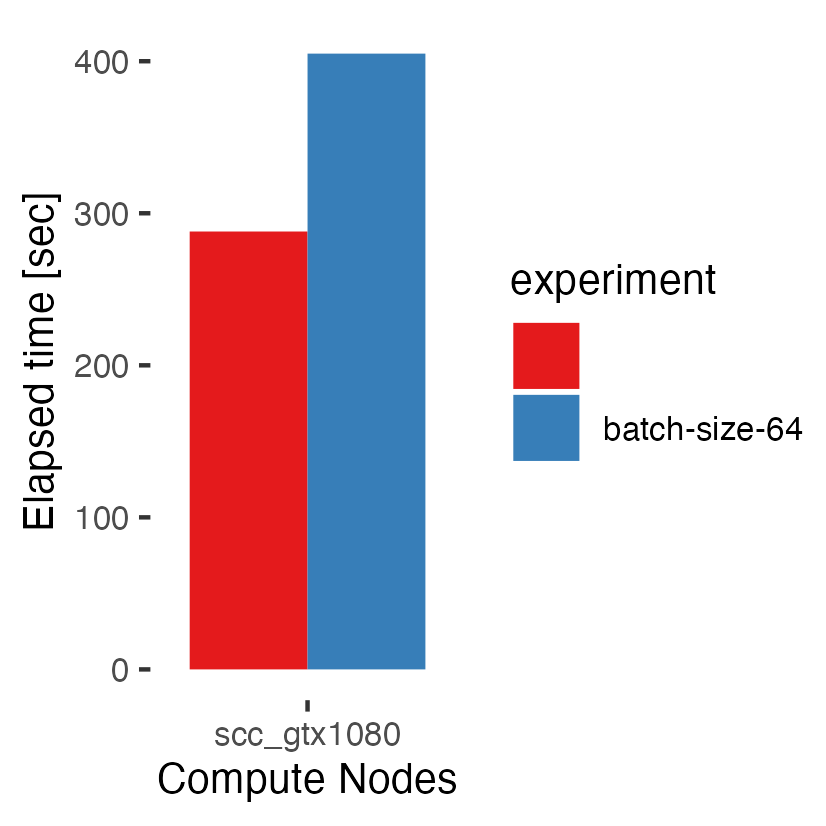
\includegraphics[width=0.85\textwidth]{../../data/sacct_barplot_by_nodes_batch-size-effect}

        \end{figure}
    \end{center}
\end{frame}

\begin{frame}[fragile]{Tensorboard}
        \footnotesize\inputminted[xleftmargin=1em,linenos,fontsize=\scriptsize, highlightlines={1,3,9-12,14-16}]{python}{../../data/tensorboard.py}
\end{frame}

\begin{frame}[fragile]{Torch profiler}
        \footnotesize\inputminted[xleftmargin=1em,linenos,fontsize=\scriptsize, highlightlines={4-10,14,15}]{python}{../../data/profiler-torch.py}
\end{frame}

\begin{frame}[fragile]{Deepspeed - FlopsProfiler}
        \footnotesize\inputminted[xleftmargin=1em,linenos,fontsize=\scriptsize, highlightlines={1,3,4,8,9,11-18}]{python}{../../data/deepspeed.py}
\end{frame}

\begin{frame}{Overview: Increased batch size (64)}
    \vspace{-1em}
\begin{center}
    \begin{figure}
        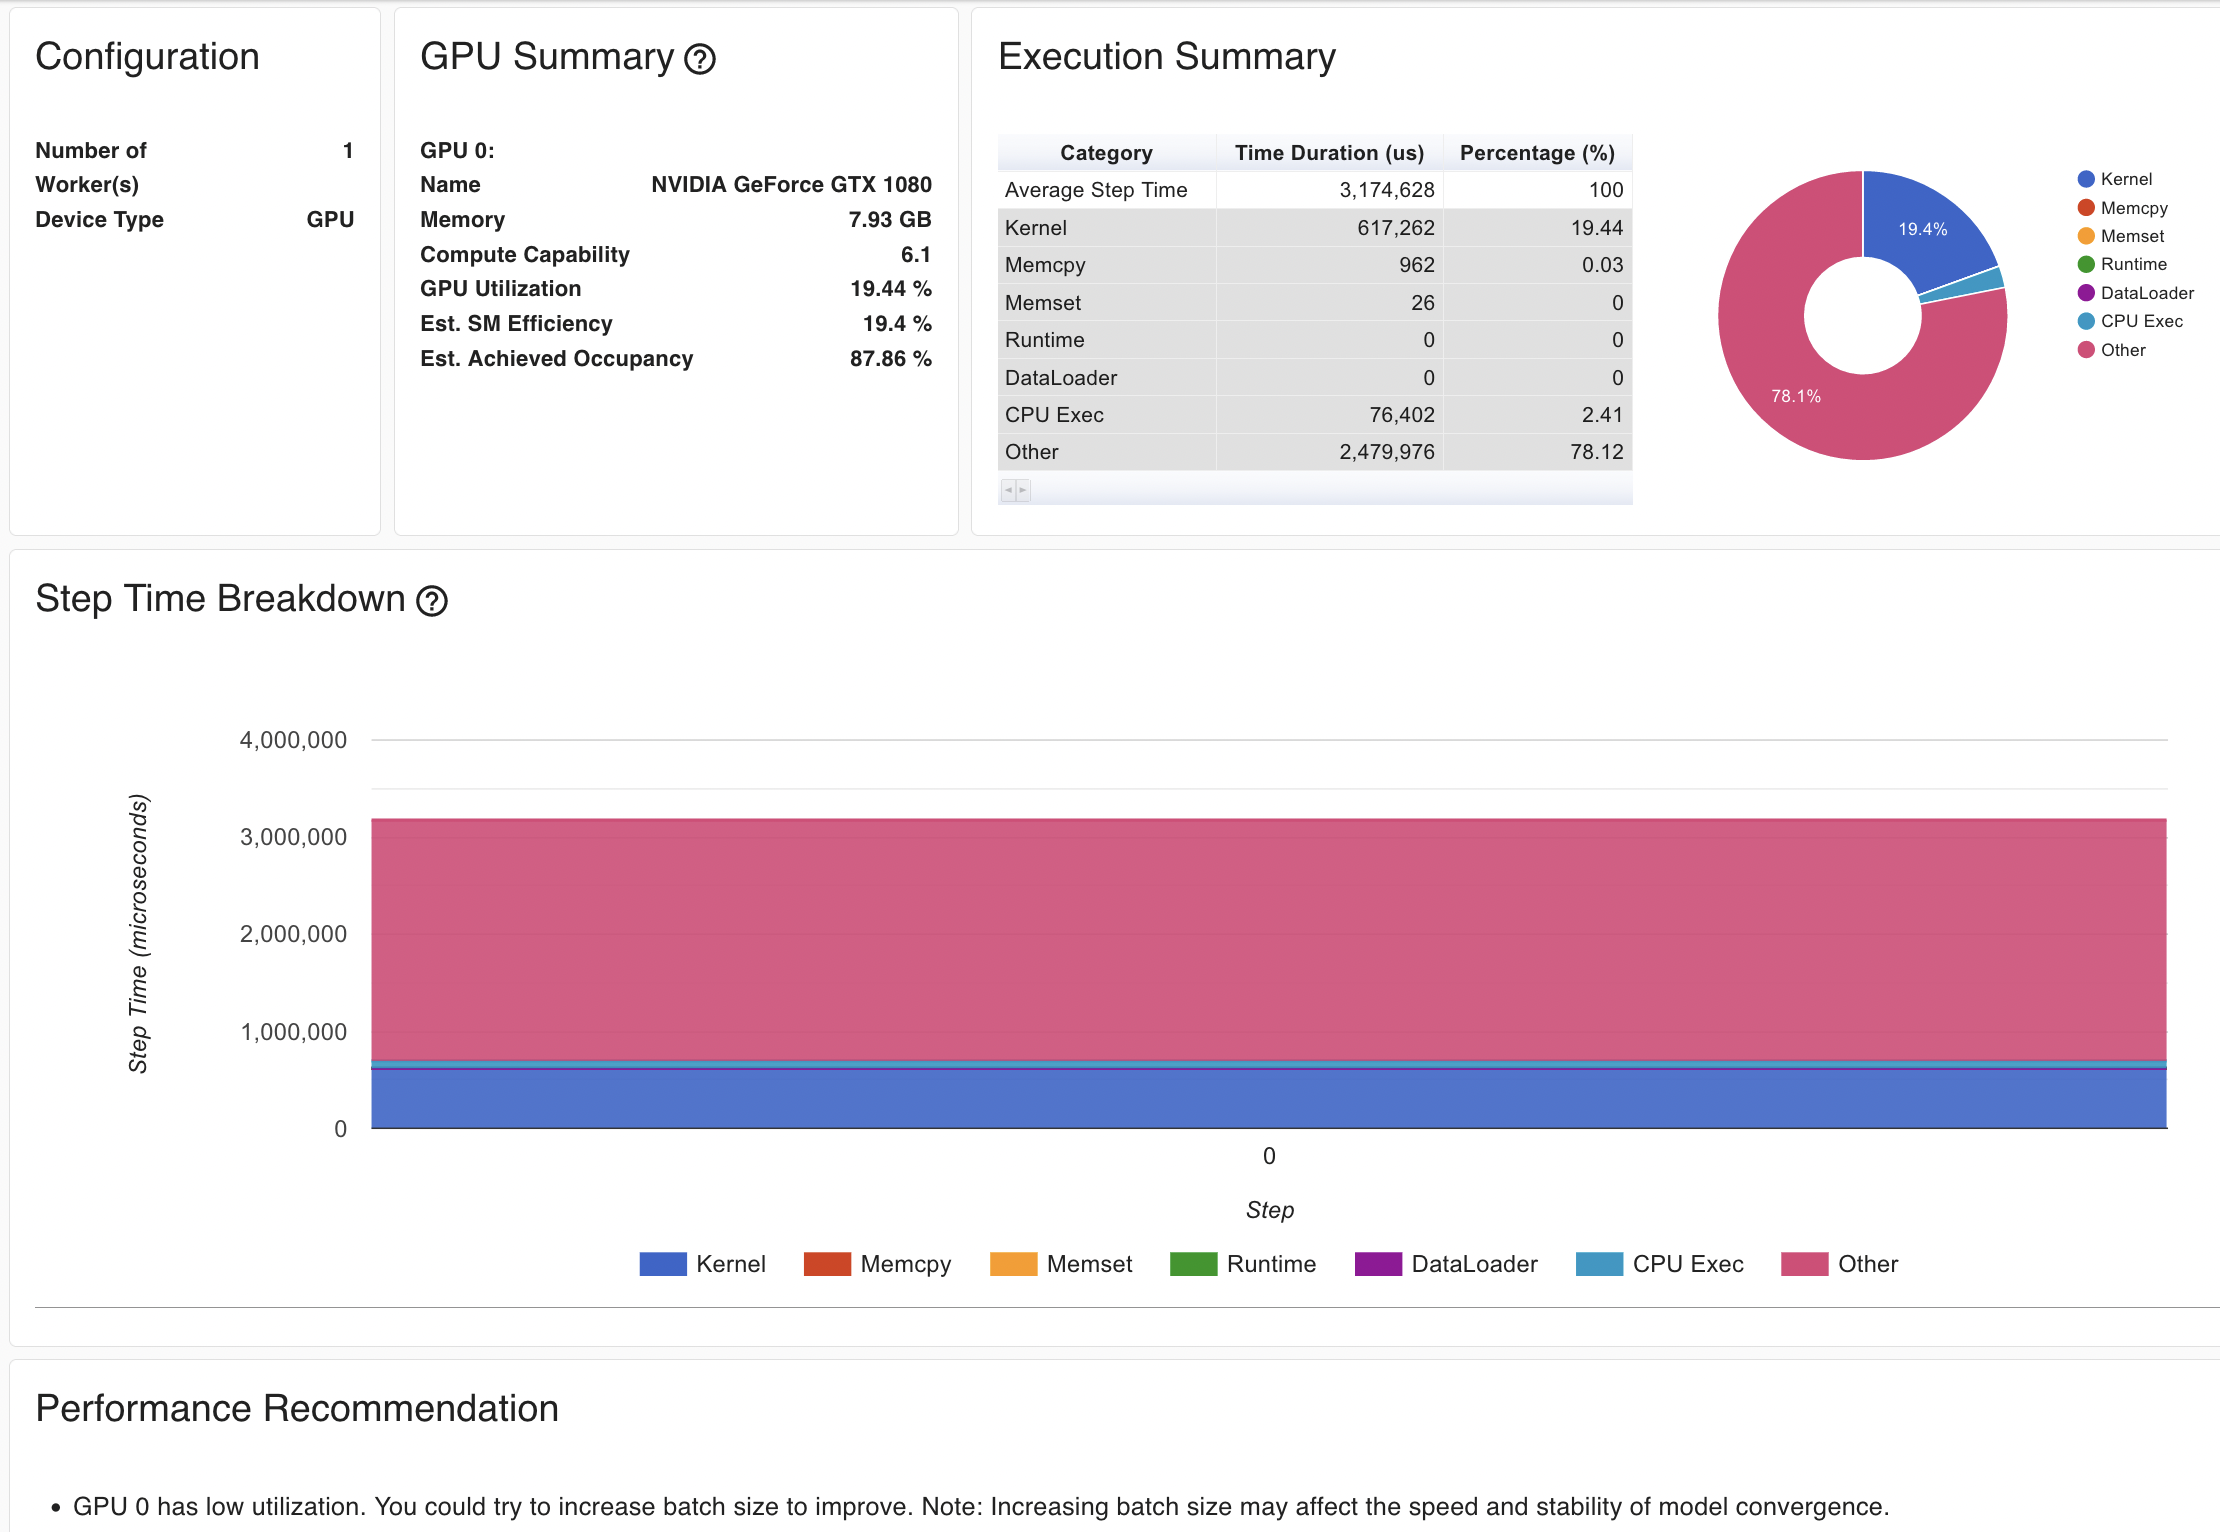
\includegraphics[width=0.7\textwidth]{../../data/scap_gtx1080_profiler-torch_batch-size-64_14650758}
    \end{figure}
    \end{center}

\end{frame}

\begin{frame}{Performance Recommendation: Increased batch size (64)}
    \vspace{-1em}
\begin{center}
    \begin{figure}
        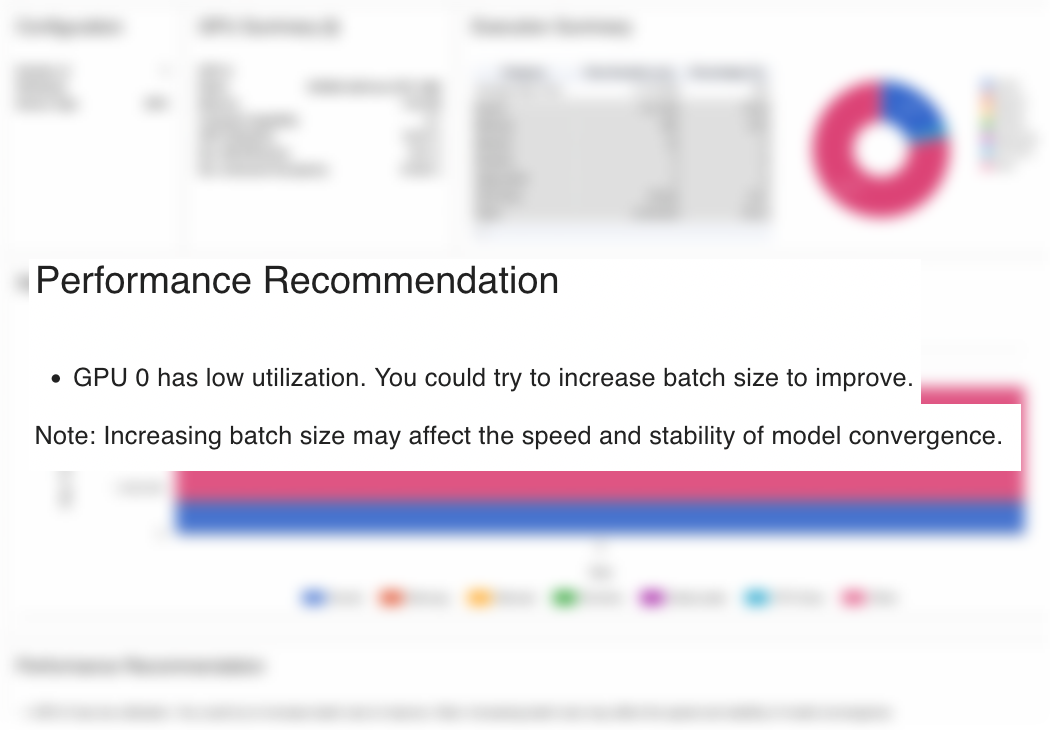
\includegraphics[width=0.7\textwidth]{../../data/scap_gtx1080_profiler-torch_batch-size-64_14650758_zoom}
    \end{figure}
    \end{center}

\end{frame}


\begin{frame}{Overview: Increased batch size (128)}
    \vspace{-1em}
\begin{center}
    \begin{figure}
        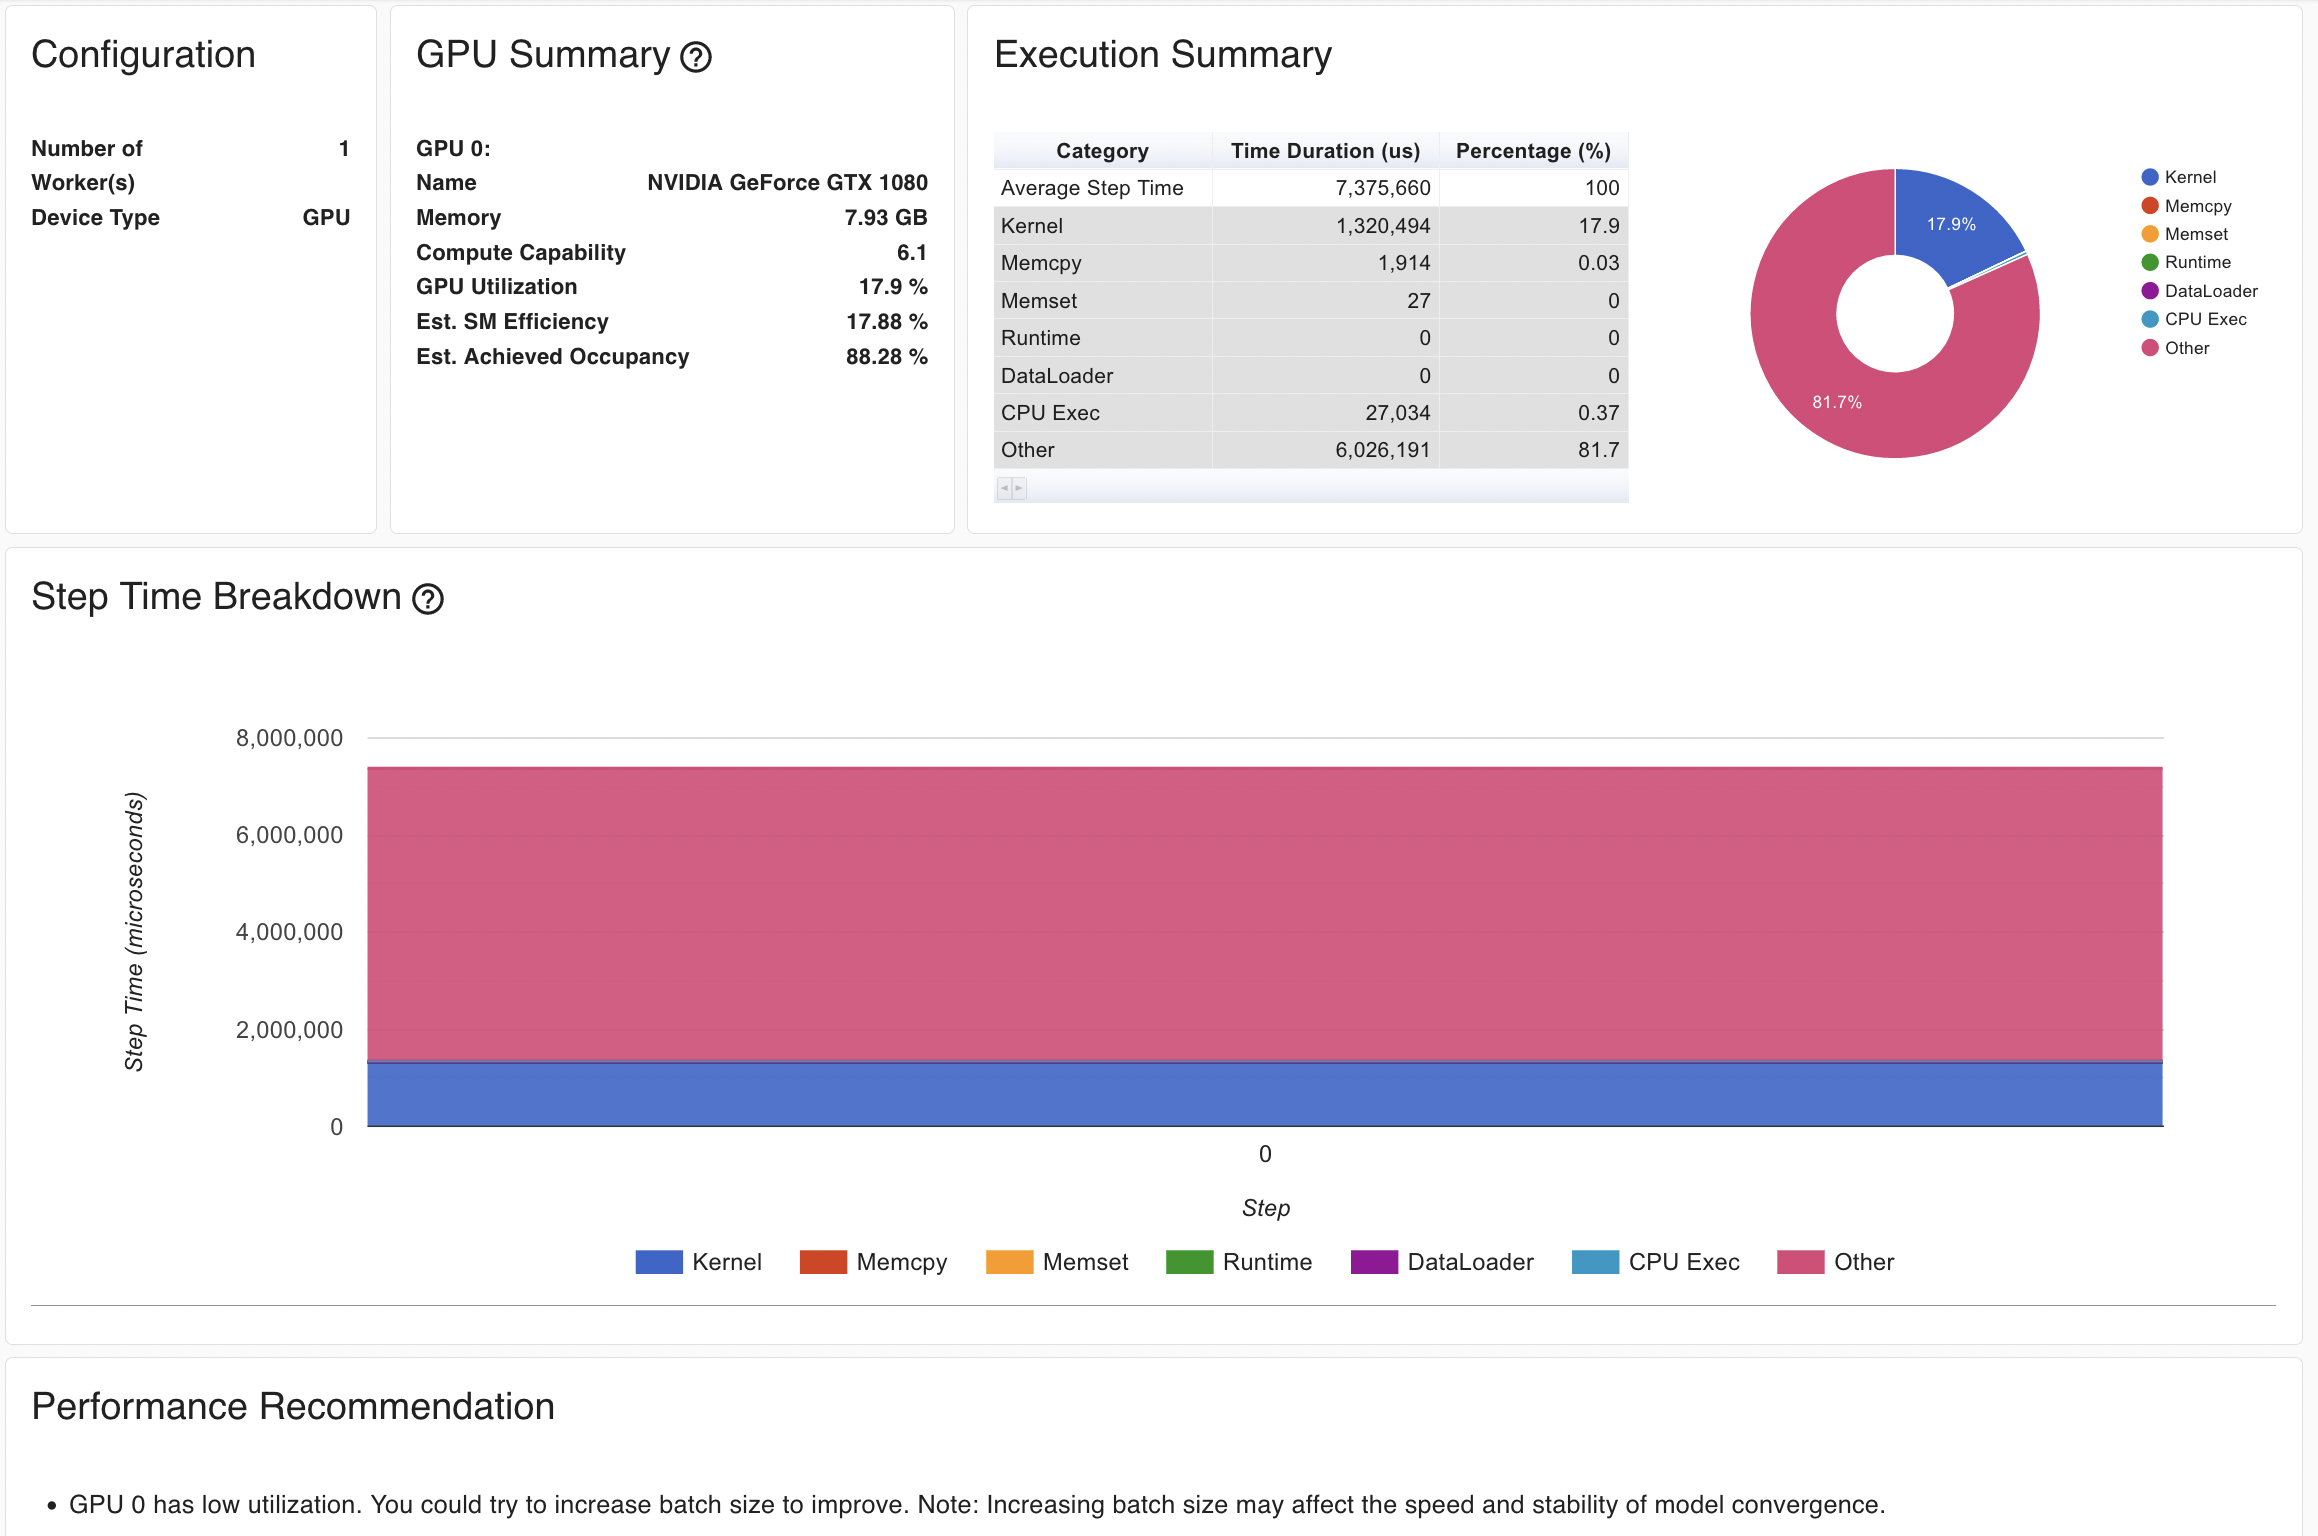
\includegraphics[width=0.7\textwidth]{../../data/scap_gtx1080_profiler-torch_batch-size-128_14650759}
    \end{figure}
    \end{center}

\end{frame}

\begin{frame}{Operator View}
    \vspace{-1em}
\begin{center}
    \begin{figure}
        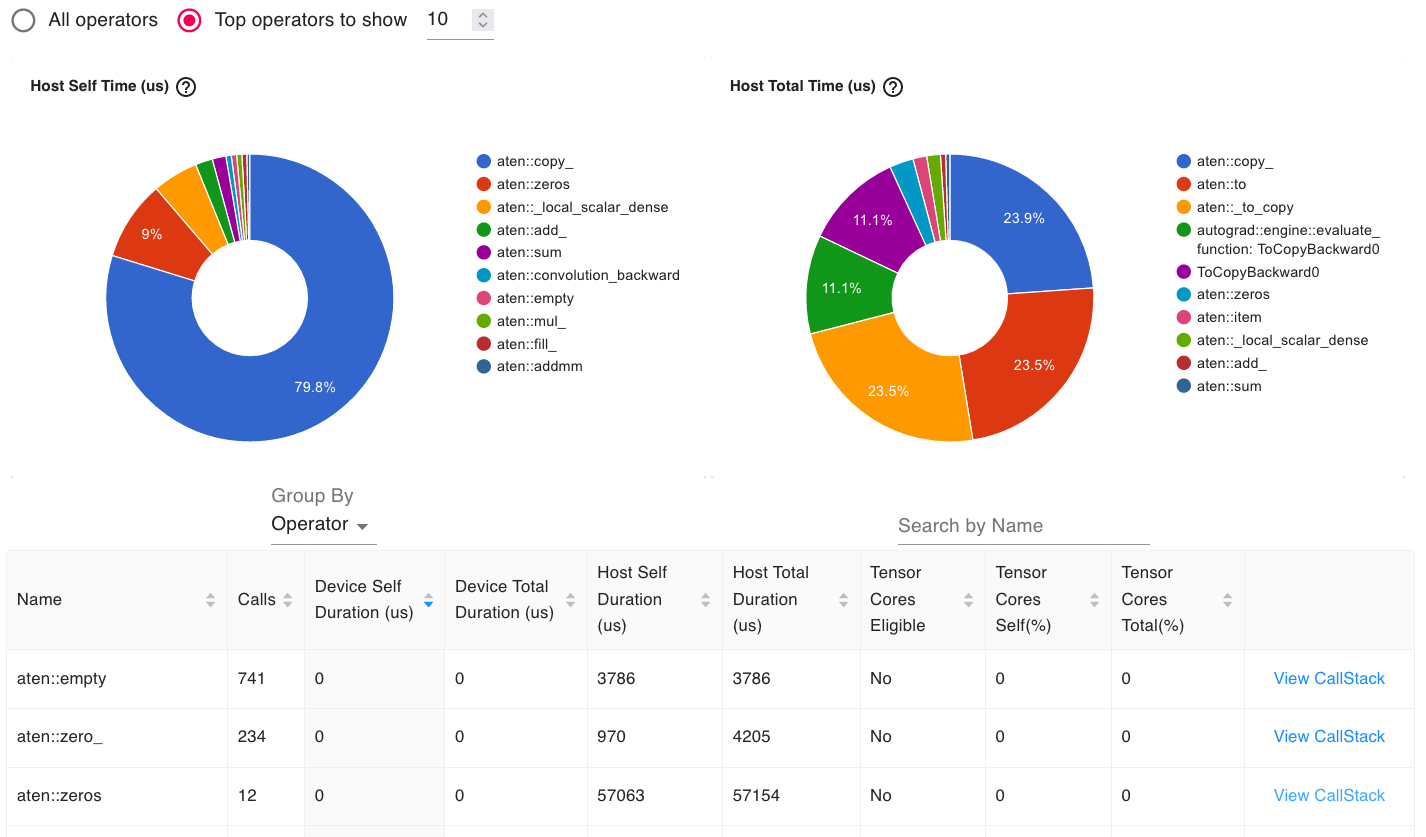
\includegraphics[width=0.9\textwidth]{../../data/scap_gtx1080_profiler-torch_batch-size-64_14650758_operator-view}
    \end{figure}
    \end{center}
\end{frame}

\begin{frame}{Operator View}
    \vspace{-1em}
\begin{center}
    \begin{figure}
        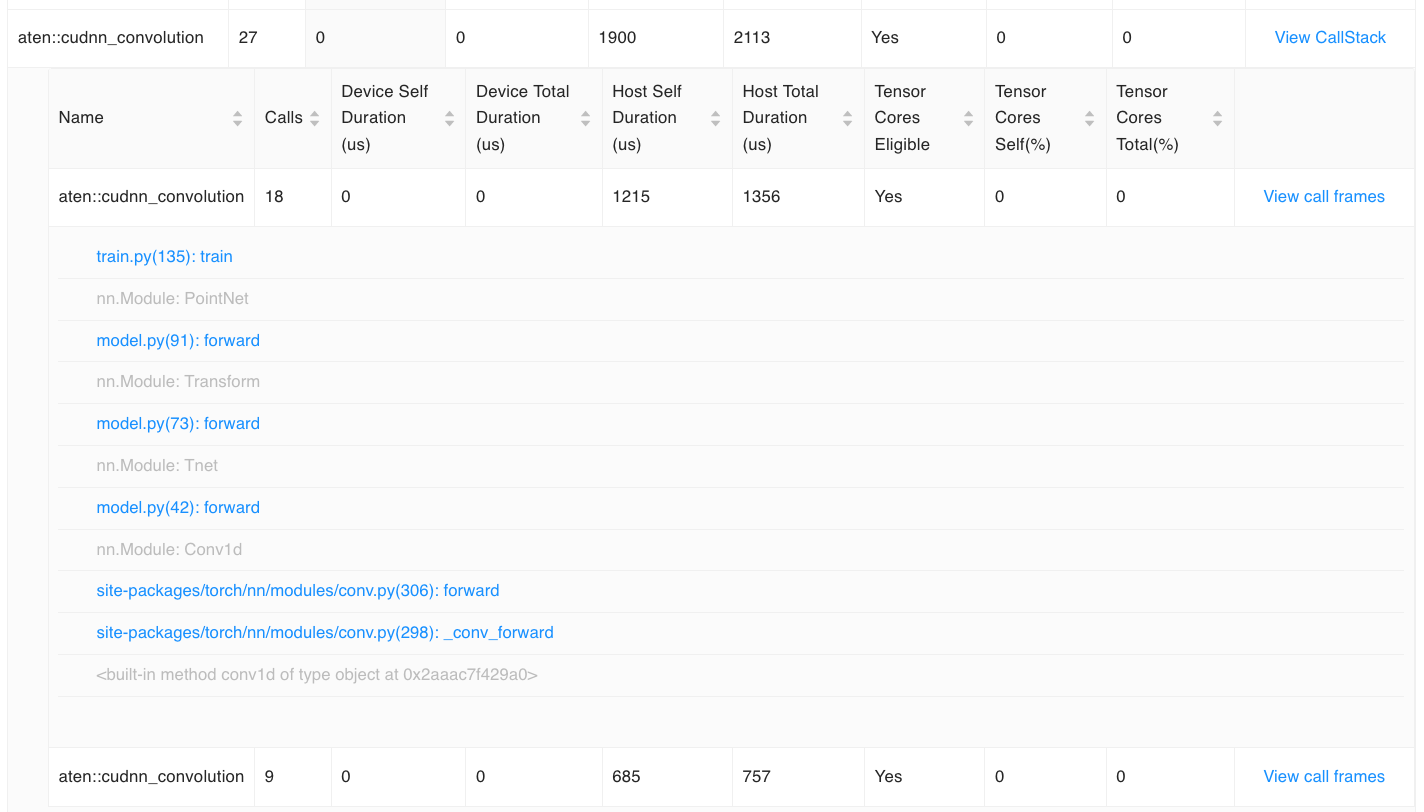
\includegraphics[width=0.9\textwidth]{../../data/scap_gtx1080_profiler-torch_batch-size-64_14650758_operator-view-details}
    \end{figure}
    \end{center}
\end{frame}

\begin{frame}{GPU Kernel View}
    \vspace{-1em}
\begin{center}
    \begin{figure}
        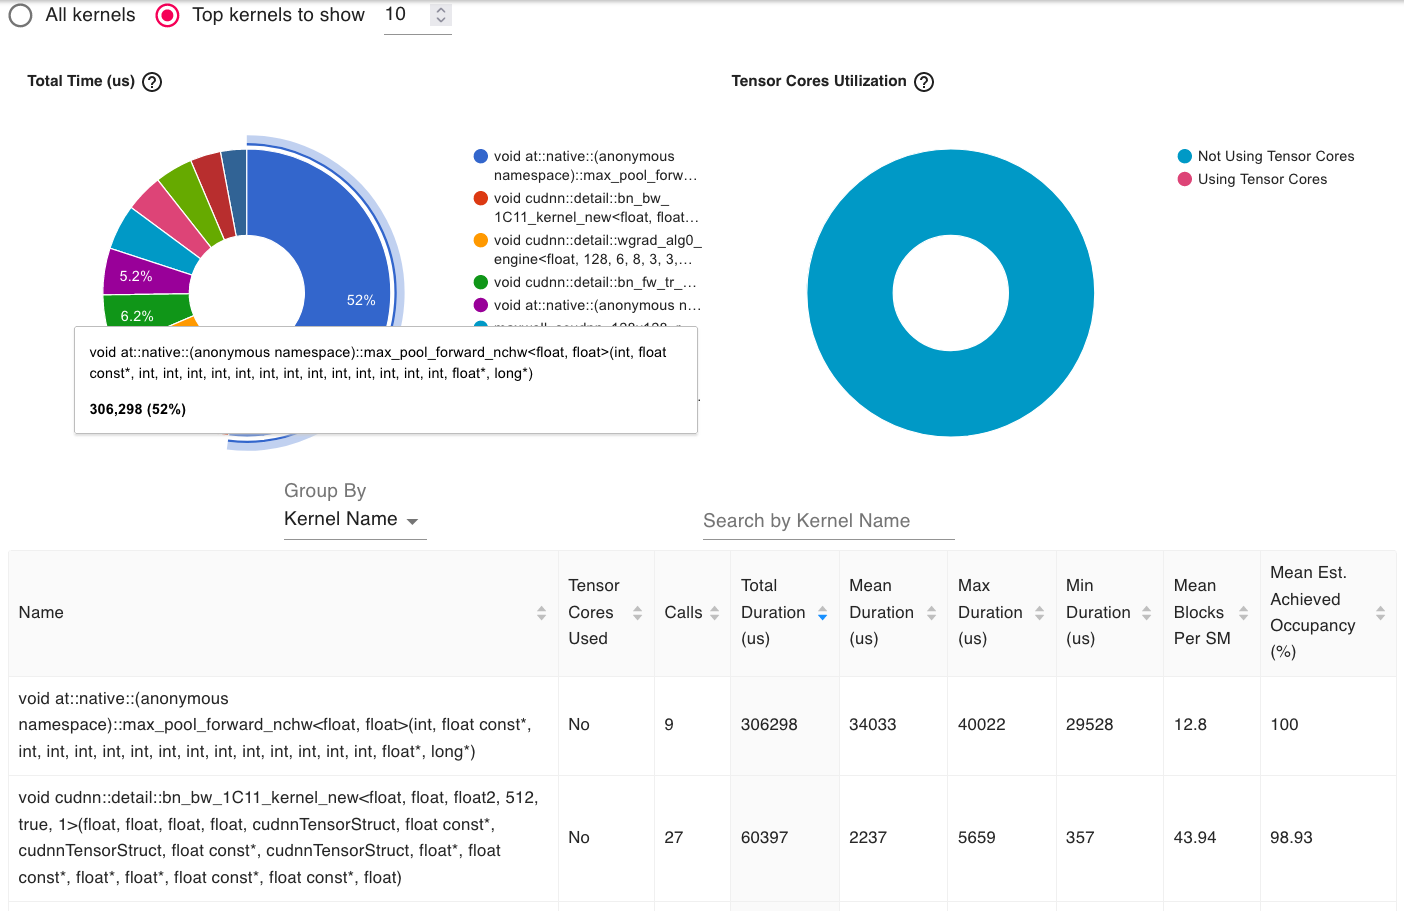
\includegraphics[width=0.9\textwidth]{../../data/scap_gtx1080_profiler-torch_batch-size-64_14650758_gpu-kernel-view}
    \end{figure}
    \end{center}
\end{frame}

\begin{frame}{Memory View}
    \vspace{-1em}
\begin{center}
    \begin{figure}
        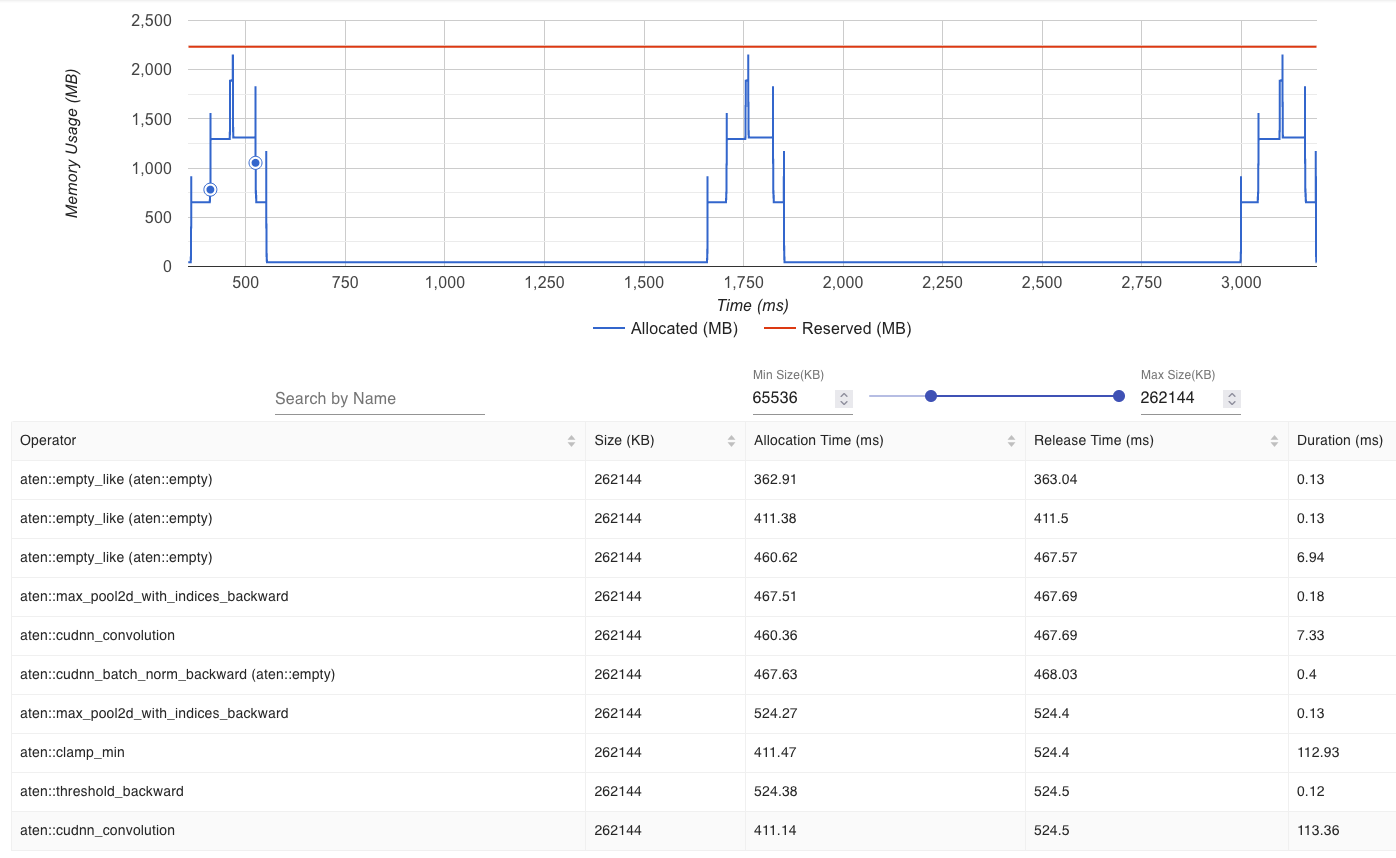
\includegraphics[width=0.85\textwidth]{../../data/scap_gtx1080_profiler-torch_batch-size-64_14650758_memory-view}
    \end{figure}
    \end{center}
\end{frame}

\begin{frame}{Module View}
    \vspace{-1em}
\begin{center}
    \begin{figure}
        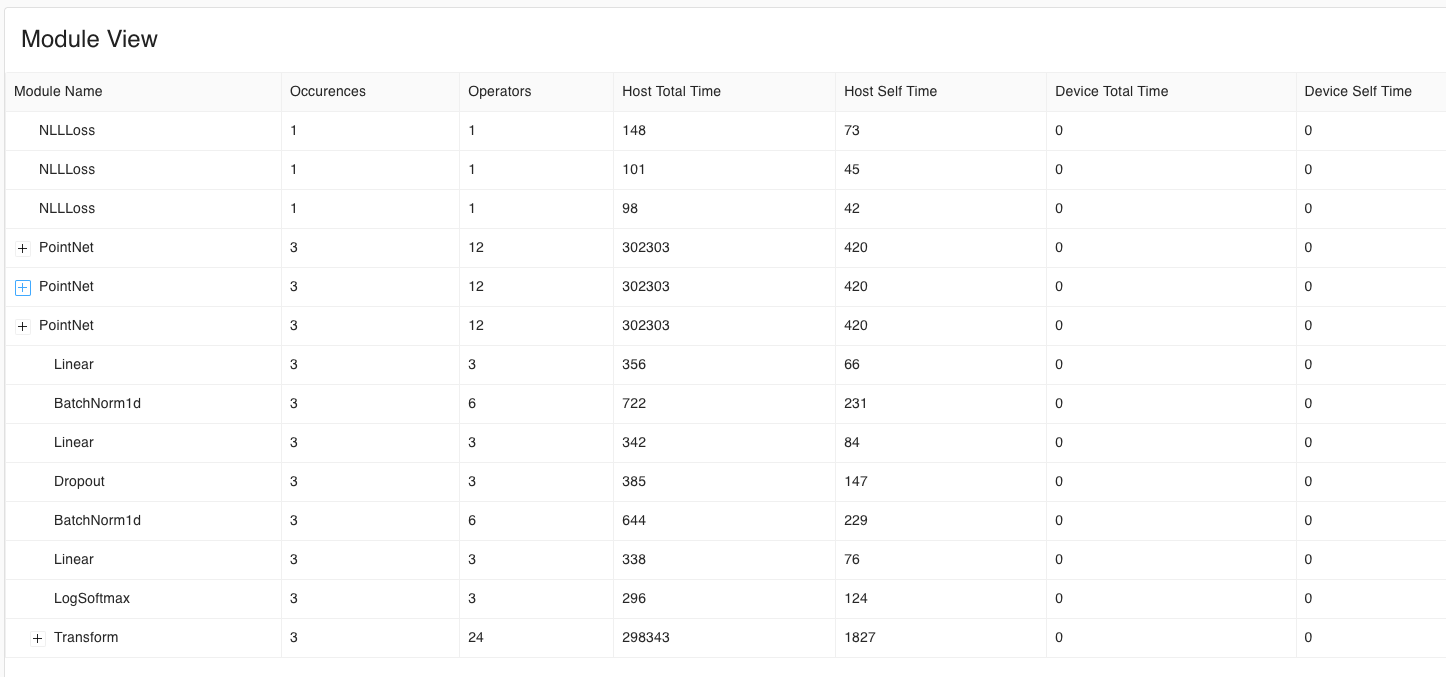
\includegraphics[width=1\textwidth]{../../data/scap_gtx1080_profiler-torch_batch-size-64_14650758_module-view}
    \end{figure}
    \end{center}
\end{frame}

\backupend

\end{document}
